\documentclass[a4paper]{article}

\usepackage{caption}
\usepackage{subcaption}
% accetta caratteri complicati tipo vocali accentate
\usepackage[T1]{fontenc}
\usepackage[utf8]{inputenc}


%collegamenti ipertestuali
\usepackage{hyperref}

%tabelle
\usepackage{booktabs}
\captionsetup[figure]{font=scriptsize}

%grafici
\usepackage{graphicx}

%matematica
\usepackage{mathtools}
\usepackage{amsmath}

%stile di pagine
\pagestyle{plain} %headings?

%Notes
\usepackage{fancyhdr}
\usepackage{wrapfig}% layout
\usepackage[export]{adjustbox}
\usepackage[colorinlistoftodos]{todonotes}						% pour faire des notes	
\usepackage[toc,page]{appendix}


\usepackage{enumerate}
\usepackage[english]{babel}
\usepackage{lmodern}
\usepackage{amsfonts,amssymb}
\usepackage[a4paper, margin=1in]{geometry}
\usepackage[parfill]{parskip}
\usepackage{epstopdf}
\usepackage{color}
\usepackage[tt]{titlepic}
\usepackage{fancyhdr}
\usepackage{enumerate}
\usepackage{lastpage}
%\usepackage{subfigure}
\usepackage{bm}
\usepackage{verbatim}
\usepackage{listings}
\usepackage{tasks}
\usepackage{float}
%\pagenumbering{gobble}



\begin{document}

\newcommand*\xbar[1]{%
  \hbox{%
    \vbox{%
      \hrule height 0.5pt % The actual bar
      \kern0.5ex%         % Distance between bar and symbol
      \hbox{%
        \kern-0.1em%      % Shortening on the left side
        \ensuremath{#1}%
        \kern-0.5em%      % Shortening on the right side
      }%
    }%
  }%
} 

%\interfootnotelinepenalty=10000
\begin{titlepage}
	\vspace{50mm}
	\begin{center}
		
\includegraphics[width=5cm]{Figures/EPFL_LOG.pdf}\\
		\vspace{2cm}
		%{\large{\bf }}\\
		\vspace{5mm}
		{\LARGE{\bf Financial Big Data Project}}\\
		\vspace{3mm}
		{\large{\bf Algorithmic Trading on FX High Frequency Data}}\\
		%\vspace{19mm} {\large{\bf }}
	\end{center}
	\vspace{60mm}
	\par
	\noindent
	%\begin{center}

			{\large{\bf Realized by: \\
            
            		\vspace{10pt}
                    
					ALESSANDRO DANIELE FORLONI\\
					MATTEO PIETROBON\\
				}}
	%\end{center}
	
	\vspace{10pt}
	\begin{center}
		{\large{\bf Academic Year\\
				2017/2018 }}
	\end{center}
\end{titlepage}

\newpage
\tableofcontents

\newpage

%COMMENTS LIKE THIS
%\todo[inline, color=red!50]{Some Comment}

%IF WE NEED TO CITE SOMETHING USE: \cite{example}.

\section{Abstract}

During the semester we learned sophisticated ways to extract information from our data and clever methods to deal with it when it is too abundant. In this project we wanted to show our skills on both those aspects, keeping in mind the important trade-off between the amount of data that we are handling and the complexity of the operations that we are performing on it.\\
In order to do that, we decided that our best option was to implement two different strategies. The first is quite basic in its principle, but it was executed on the overwhelming amount of data that we collected. The other strategy allowed us to showcase a deeper financial intuition, but, due to the higher computational burden, we only applied it to the last part of the data we downloaded.


\section{Introduction}

We tried to structure our report in a narrative way, presenting both the issues that we faced and the solutions that we applied. As mentioned in the abstract, we developed two different strategies for our project. Both strategies use the same data, high-frequency FX data. Their rationale and results are quite independent and will, therefore, be presented separately.\\
All our strategies are built through adapted processes, i.e. we only use past information to make decisions.\\ 


\section{Data Description}

We decided to use FX high-frequency data because of its abundance and because of our personal interest in this field. We focused on 5 currency pairs:
\begin{itemize}
\item EUR / USD
\item EUR / CHF
\item EUR / GBP
\item EUR / JPY
\item EUR / AUD
\end{itemize}
The time series start on January $1^{\text{st}}$ 2003 and end on December $31^{\text{st}}$ 2016 and it provides Bid and Ask prices for each pair. The data was stored tick-by-tick and grouped in monthly \emph{csv} files, whose size was obviously changing month-by-month.\\
We downloaded the same data for the first 11 months of 2017 and used it to test out-of-sample our strategies.


\subsection{Downloading the data} 

We downloaded the data from this \href{http://www.histdata.com/download-free-forex-historical-data/?/ascii/tick-data-quotes}{Website}. It provides free high-frequency FX data for several currency pairs. We chose the longest series that had EUR as a common reference.\\
We had to download a different file for every currency pair, year and month (5 x 14 x 12 = 840, not even counting the 2017 files). Therefore, we decided to automate the process. However, we could not just access the files through an \emph{url}, the 'download' link was a javascript on the web page so we had to use the \emph{Selenium} package to click on it. We ran this script overnight and stored the data locally. \\
We finally had 895 files, with a total size of 25.1 Gb. The whole process took around 5 hours.

\subsection{Data wrangling} 

We decided to keep our series separate because our strategies were not exploiting cross-currency relations. We aggregated the files by year, but kept the separation into months within them thanks to the structure of \emph{hdf} files.\\
We noticed that the original files were composed of a column with the timestamp, the Bid price, the Ask price and a column of zeros. We removed the last column and transformed the timestamp in a datetime object, that is easier to handle in Python.\\
We checked a portion of the data for the presence of \emph{NaN}s but we could not find any, nonetheless we included a command to drop all the rows which might have contained them. We also checked for the presence of outliers and we found around 10 of them for GBP, CHF and JPY in 2004. They might have been flash crashes but we could find no reference to them in the news and decided to drop those entries. The data after 2004 seems to be much more reliable.\\
Another issue that we found was that the order of the Bid and the Ask column was reversed in June 2009. This was quite easy to solve, but harder to spot because it was not mentioned in the website that we used to download the data.\\
Finally, we have no data during the weekends.\\
We stored the data in \emph{hdf} format, in this way the datetime object was preserved. Finally we had 75 files with a total size of around 17.5 Gb. The whole process took around 1 hour.

\subsection{Descriptive Statistics} 

In Figure \ref{fig:1}, \ref{fig:2}, \ref{fig:3}, \ref{fig:4}, \ref{fig:5} and \ref{fig:6} we report some of the descriptive statistics for the resulting data. We can see that the amount of transactions per year is steadily increasing, reflecting the digitalization of the process. Moreover, we can see that the price process is relatively stable and the drift is close to zero, this is typical of FX data.\\
Please note that we have not examined the testing data.

\begin{figure}
	\centering
	\begin{minipage}{.5\textwidth}
		\centering
		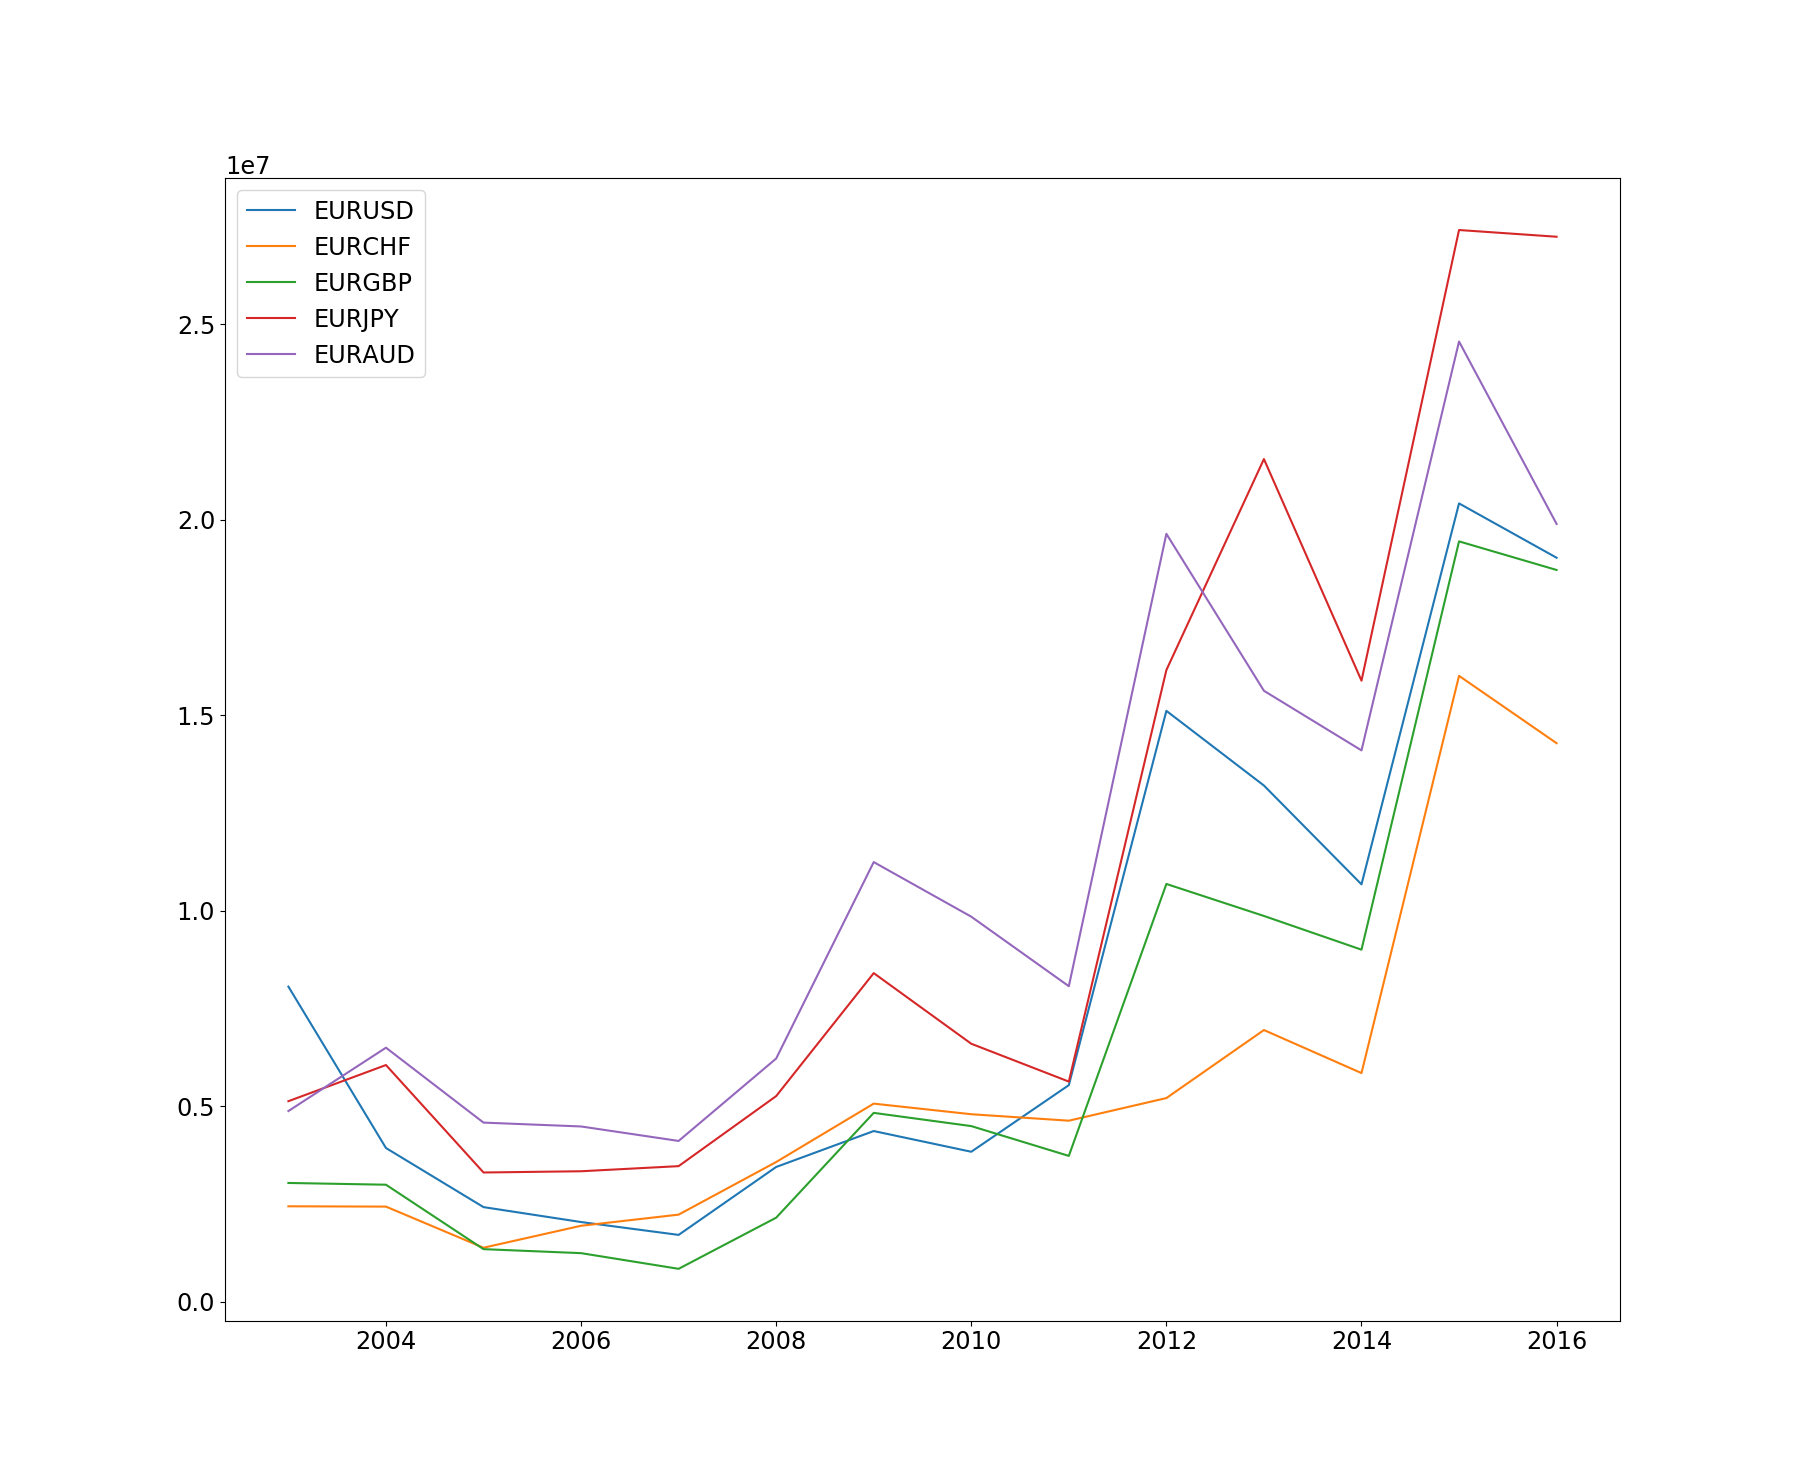
\includegraphics[width=\linewidth]{Figures/counts}
		\captionof{figure}{Data Entries by Currency each Year}
		\label{fig:1}
	\end{minipage}%
	\begin{minipage}{.5\textwidth}
		\centering
		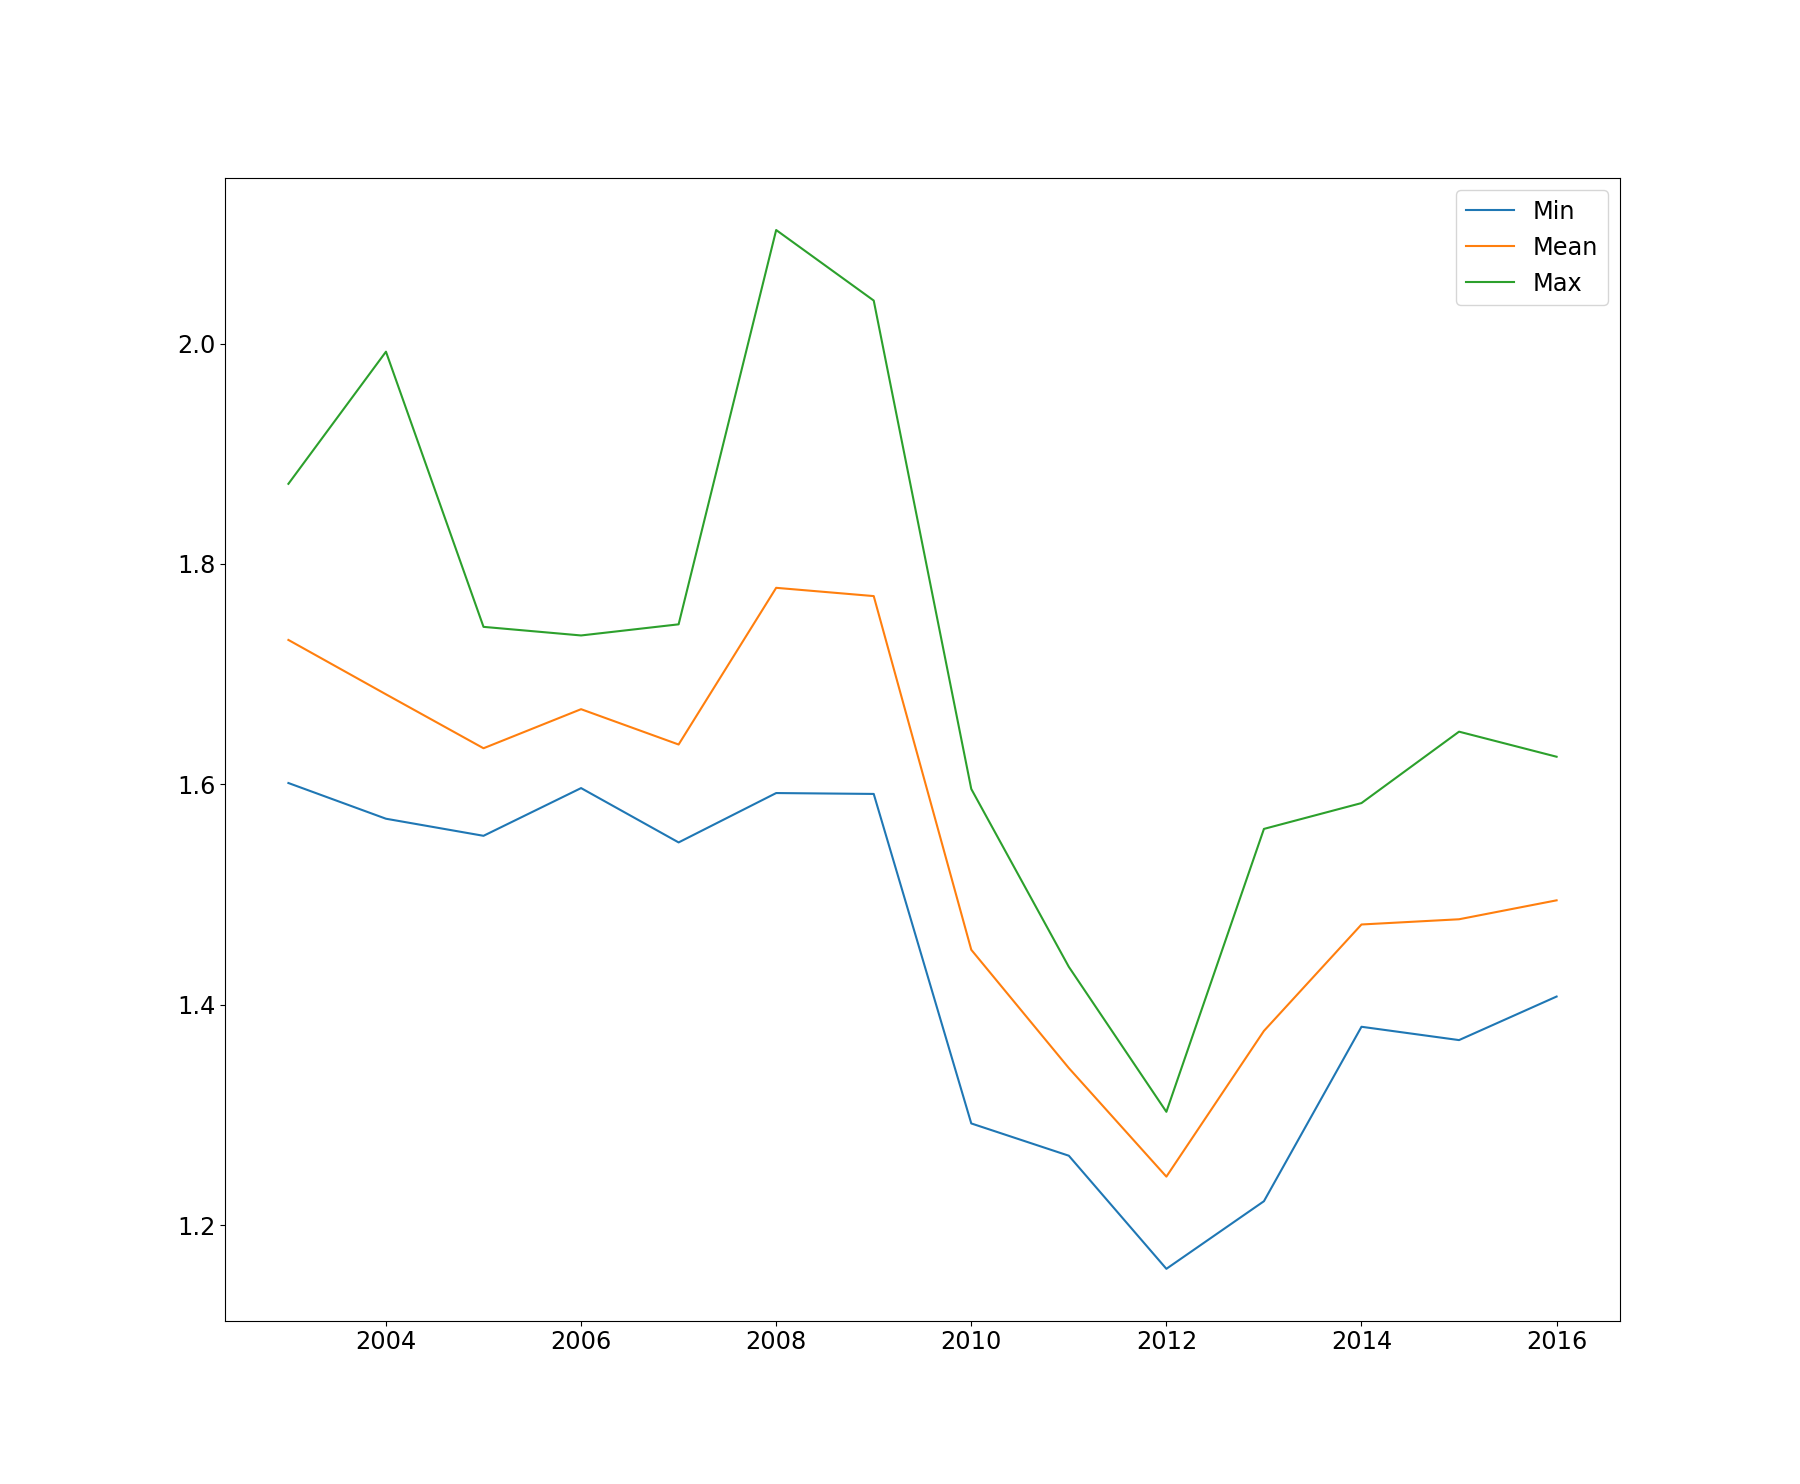
\includegraphics[width=\linewidth]{Figures/stats_aud}
		\captionof{figure}{Min, Mean and Max of EURAUD each year}
		\label{fig:2}
	\end{minipage}
	\begin{minipage}{.5\textwidth}
	\centering
	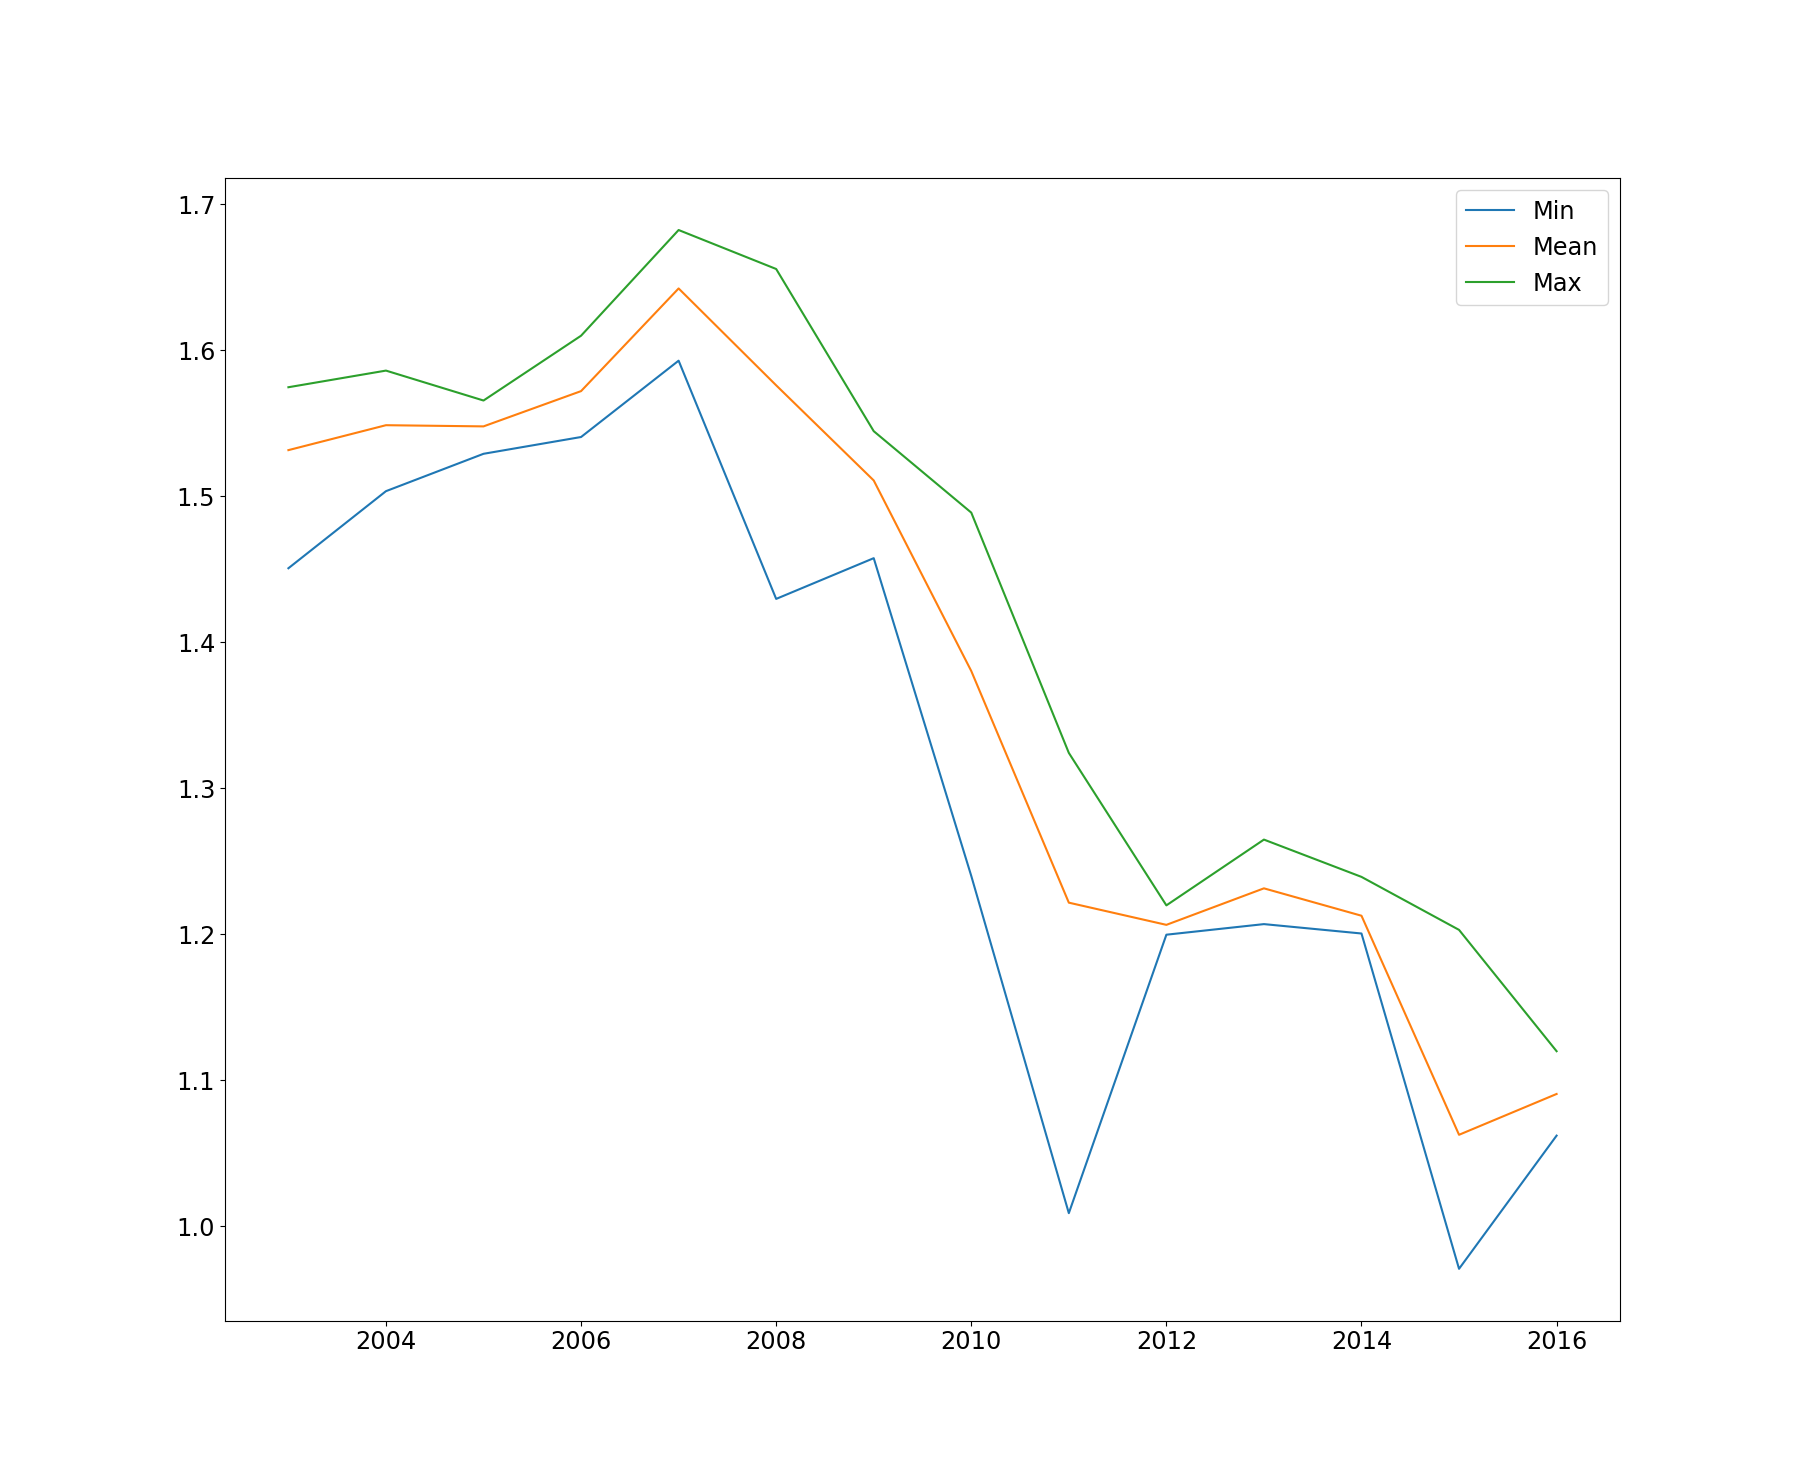
\includegraphics[width=\linewidth]{Figures/stats_chf}
	\captionof{figure}{Min, Mean and Max of EURCHF each year}
	\label{fig:3}
	\end{minipage}%
	\begin{minipage}{.5\textwidth}
	\centering
	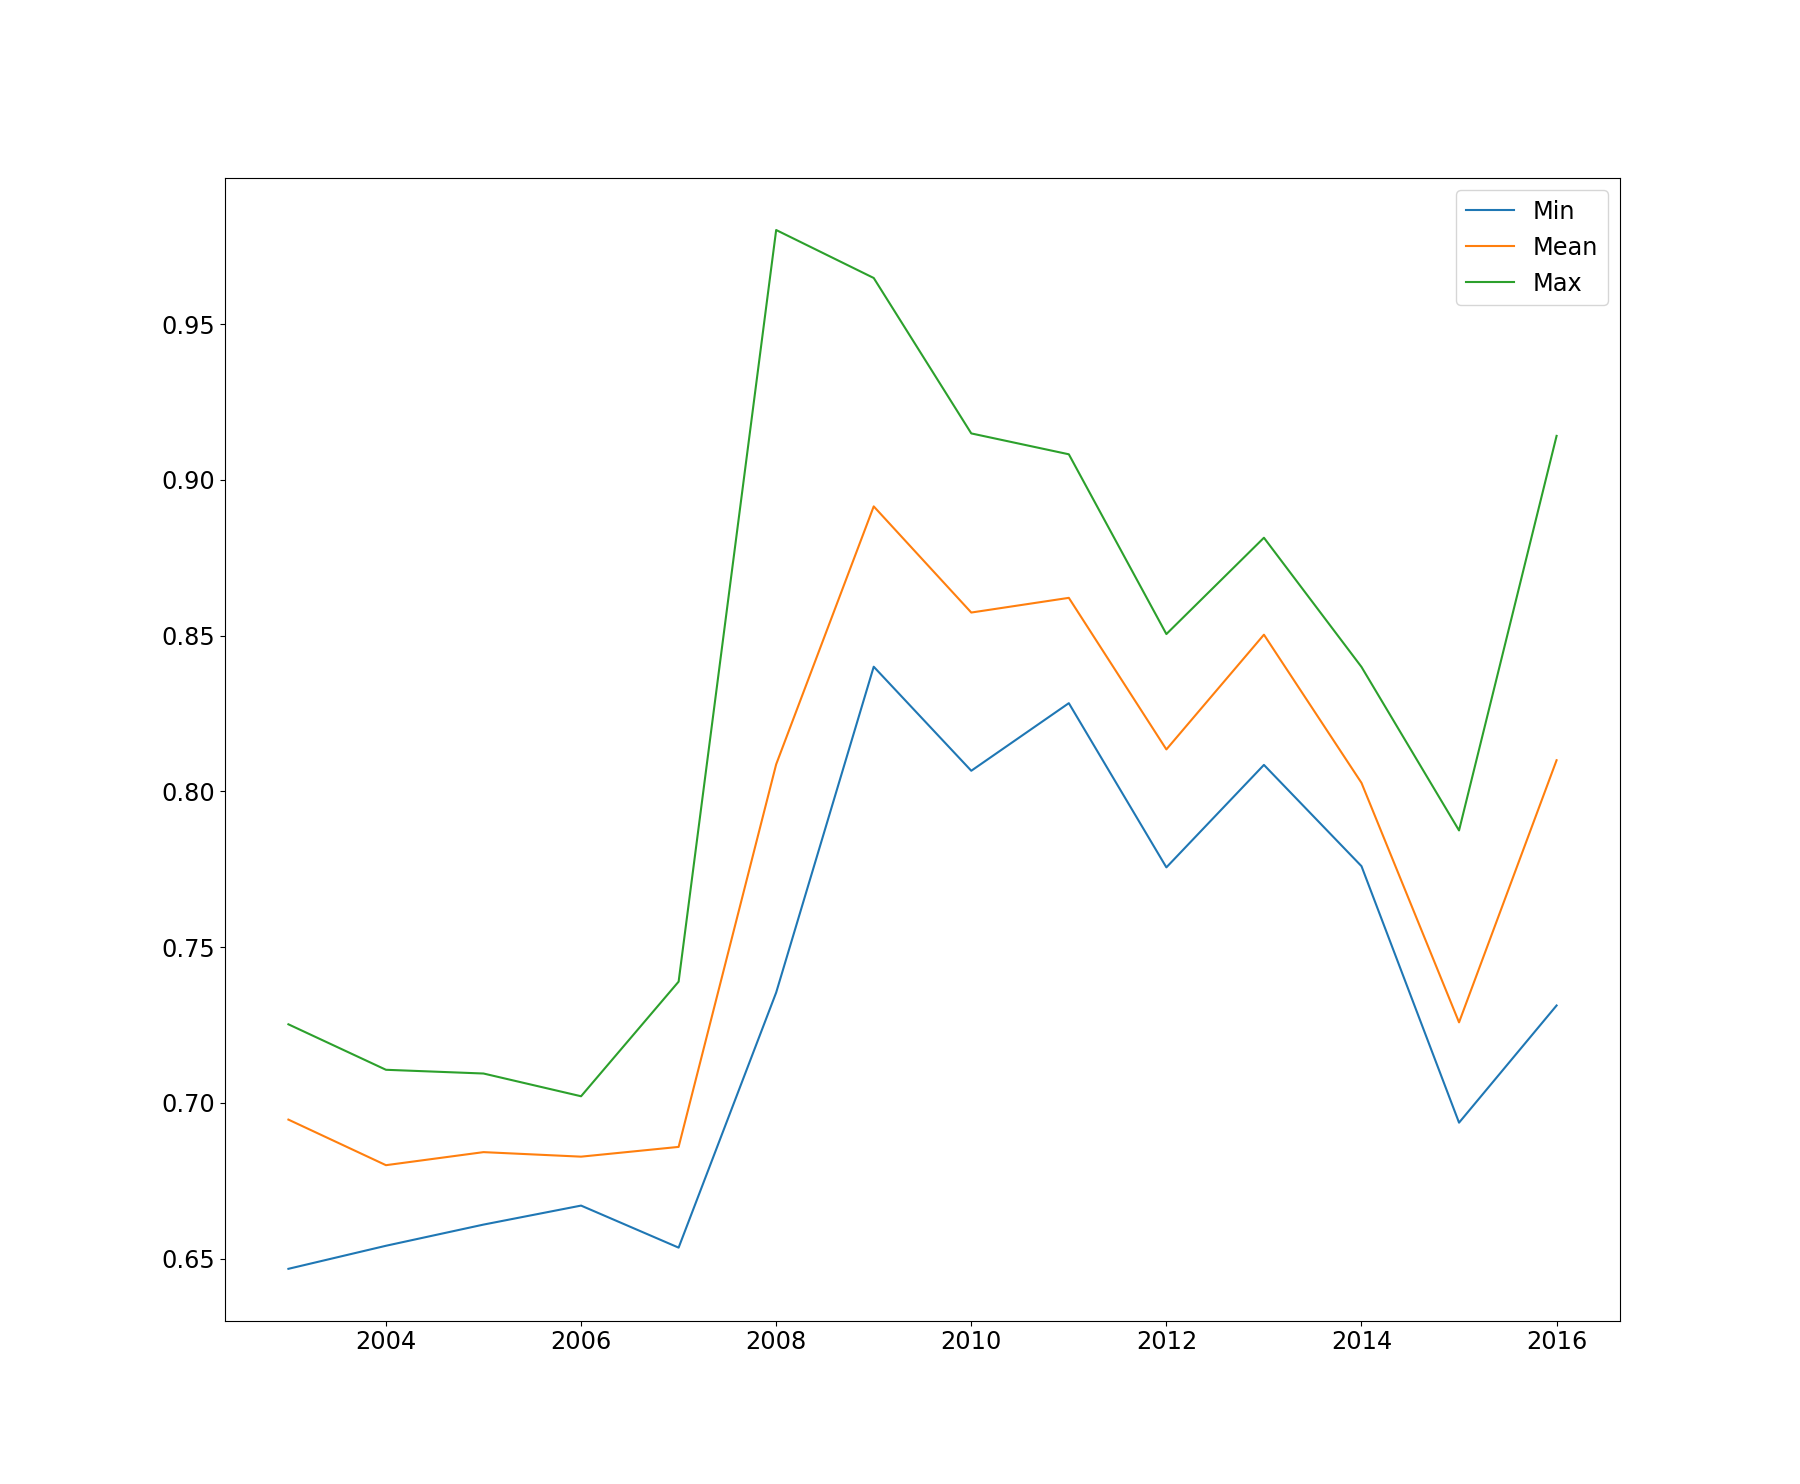
\includegraphics[width=\linewidth]{Figures/stats_gbp}
	\captionof{figure}{Min, Mean and Max of EURGBP each year}
	\label{fig:4}
	\end{minipage}
	\begin{minipage}{.5\textwidth}
	\centering
	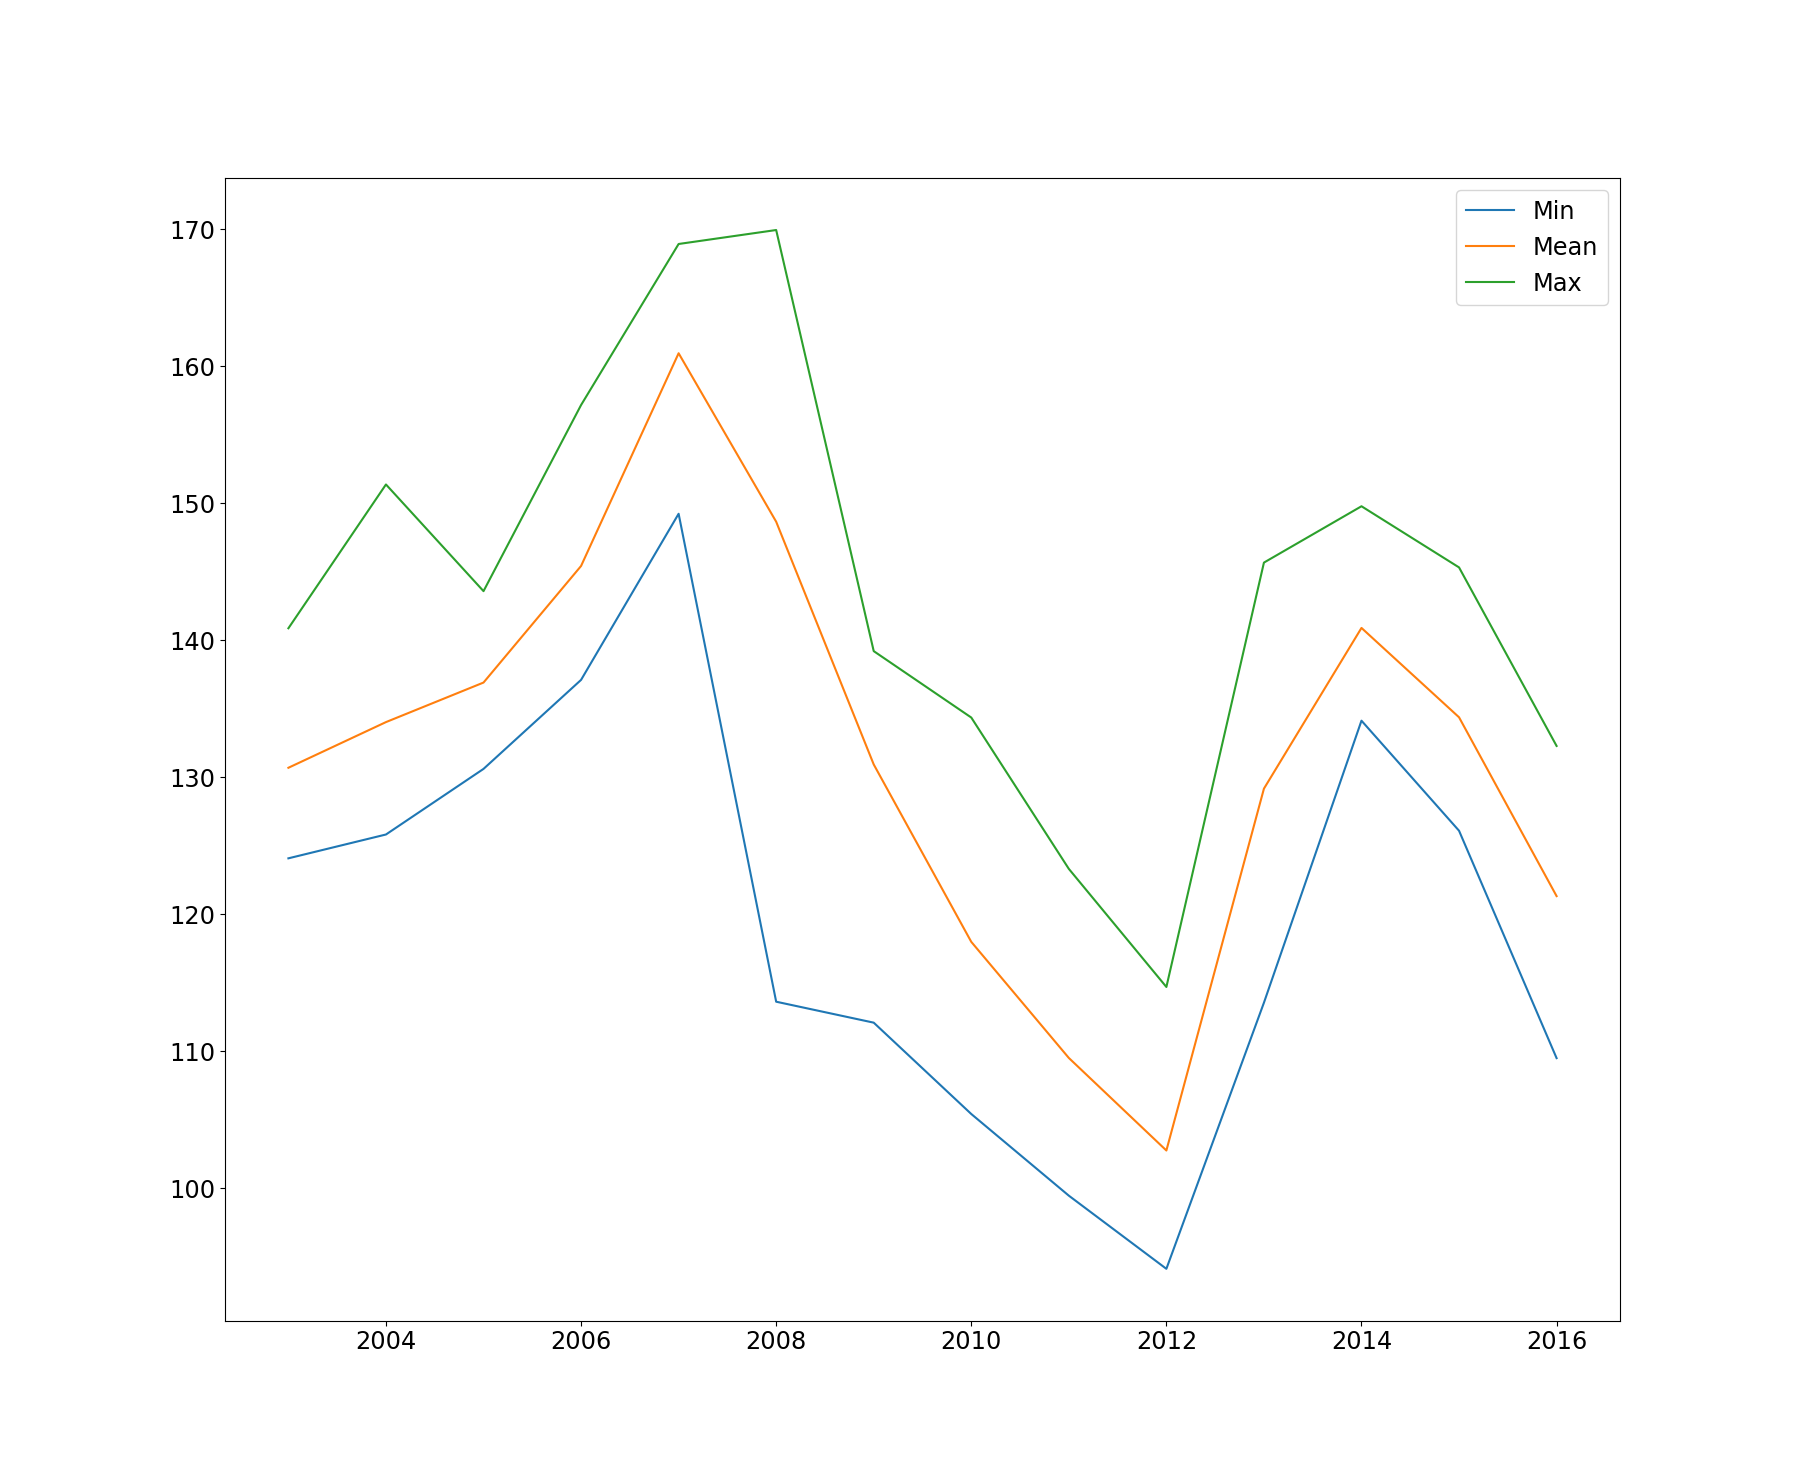
\includegraphics[width=\linewidth]{Figures/stats_jpy}
	\captionof{figure}{Min, Mean and Max of EURJPY each year}
	\label{fig:5}
	\end{minipage}%
	\begin{minipage}{.5\textwidth}
	\centering
	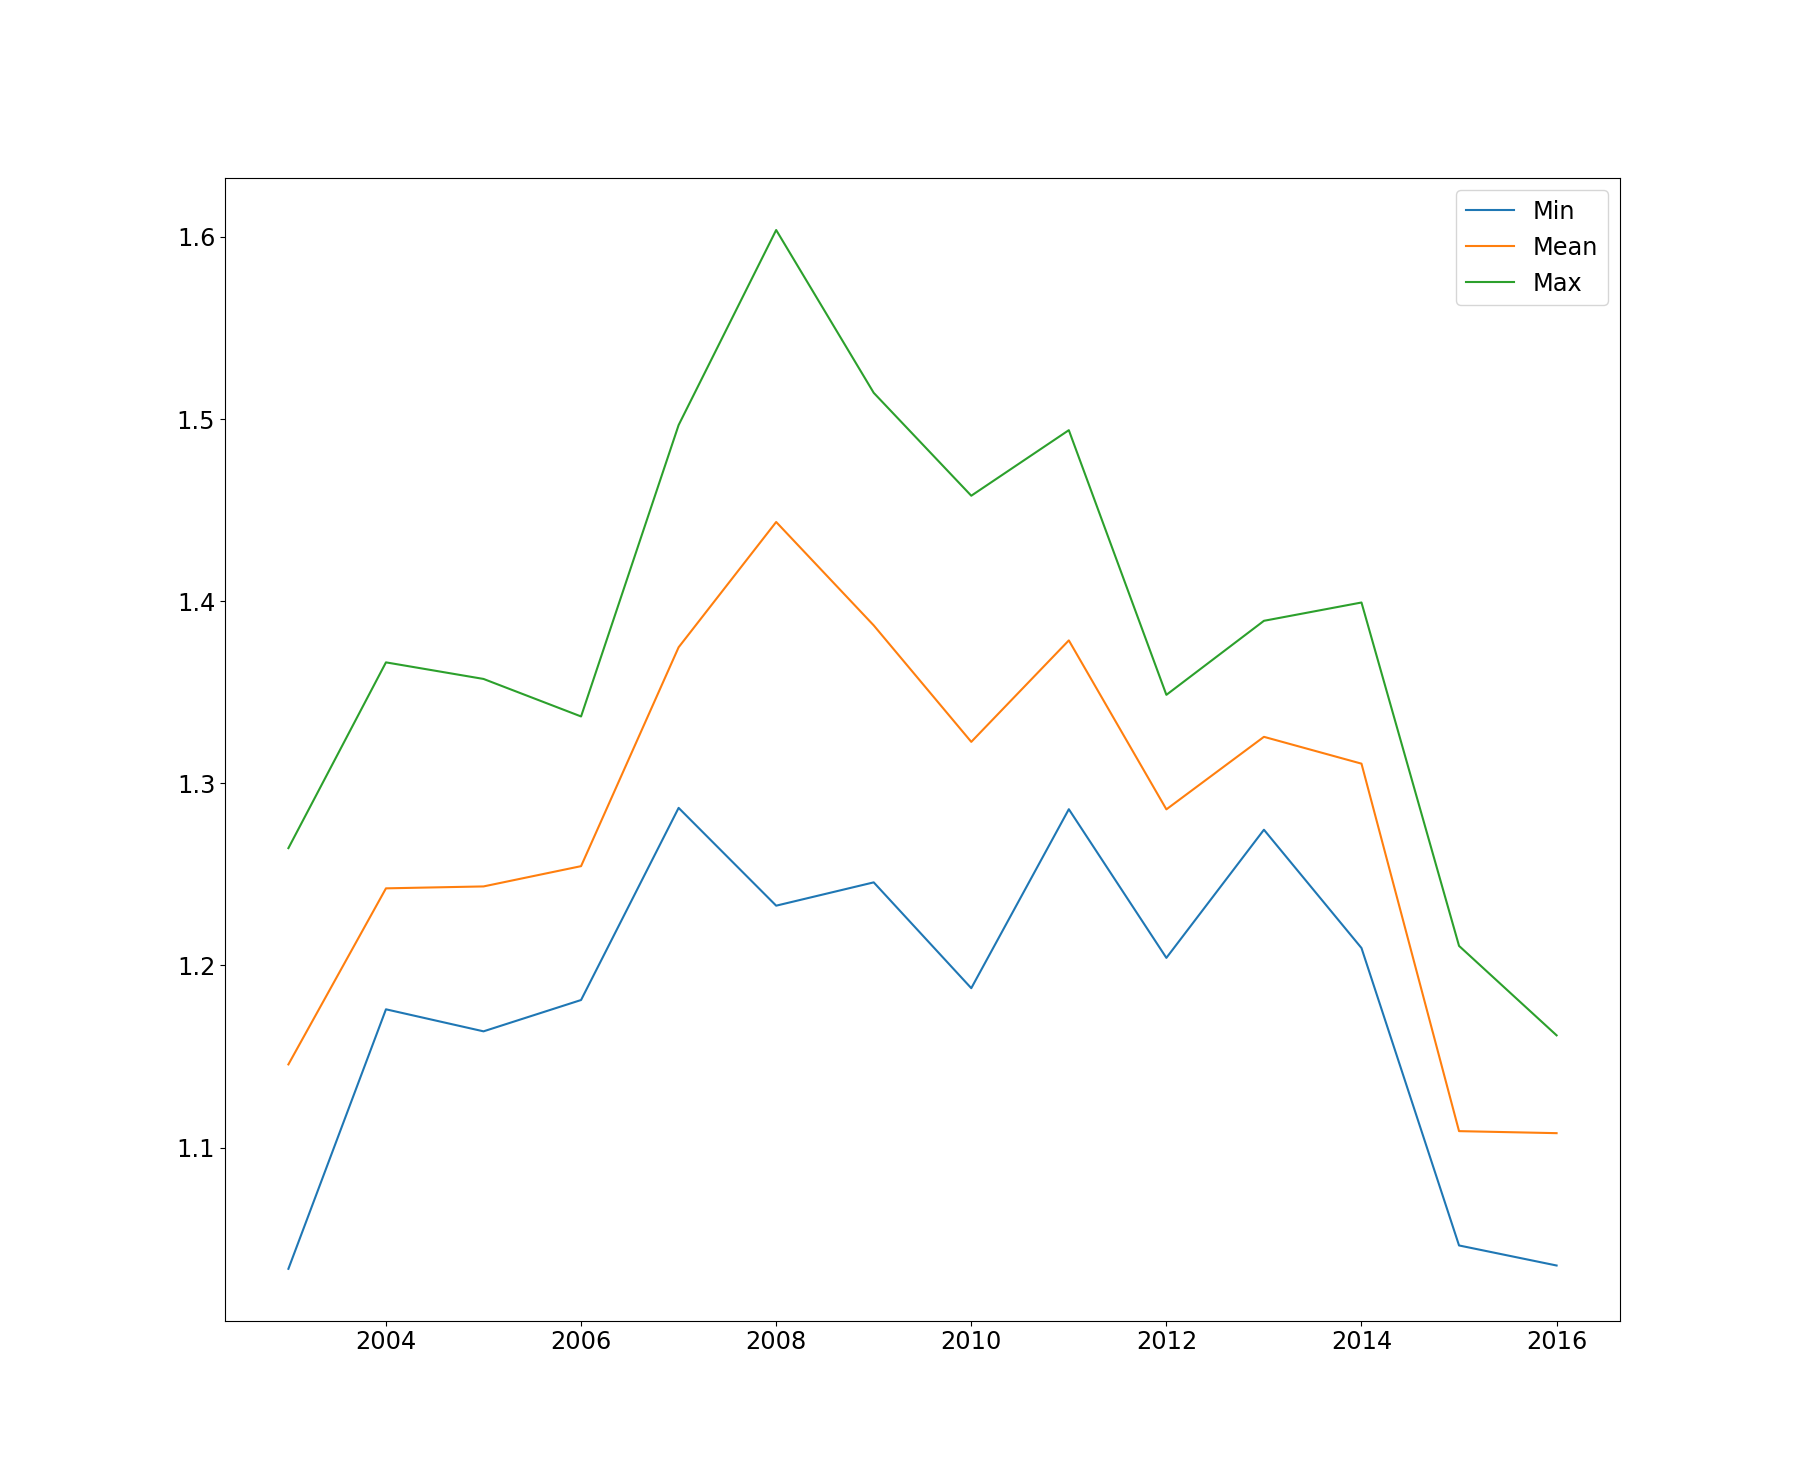
\includegraphics[width=\linewidth]{Figures/stats_usd}
	\captionof{figure}{Min, Mean and Max of EURUSD each year}
	\label{fig:6}
	\end{minipage}
\end{figure}


\section{Mean Reversion Strategy}

The FX environment is famous for its mean reverting properties. We tried to exploit them by developing this strategy. The main idea behind it is that the price process is quite stable and, when a big event happens, the market can overreact and will then return to a more balanced level. Since we are only looking at the price process, our approach is very limited because we must decide whether there was an overshoot just from the magnitude of the shock and this is not trivial.\\
In Figure \ref{fig:7} and \ref{fig:8} we report two extreme cases of what we have just said. In Figure \ref{fig:7} the mean reversion effect is almost not present, the jumps are neat and they are not followed by a recall. In Figure \ref{fig:8}, on the contrary, we have some nice oscillations that we managed to exploit. The two lines that we plotted are the Bid and the Ask.

\begin{figure}[h]
	\centering
	\begin{minipage}{.5\textwidth}
		\centering
		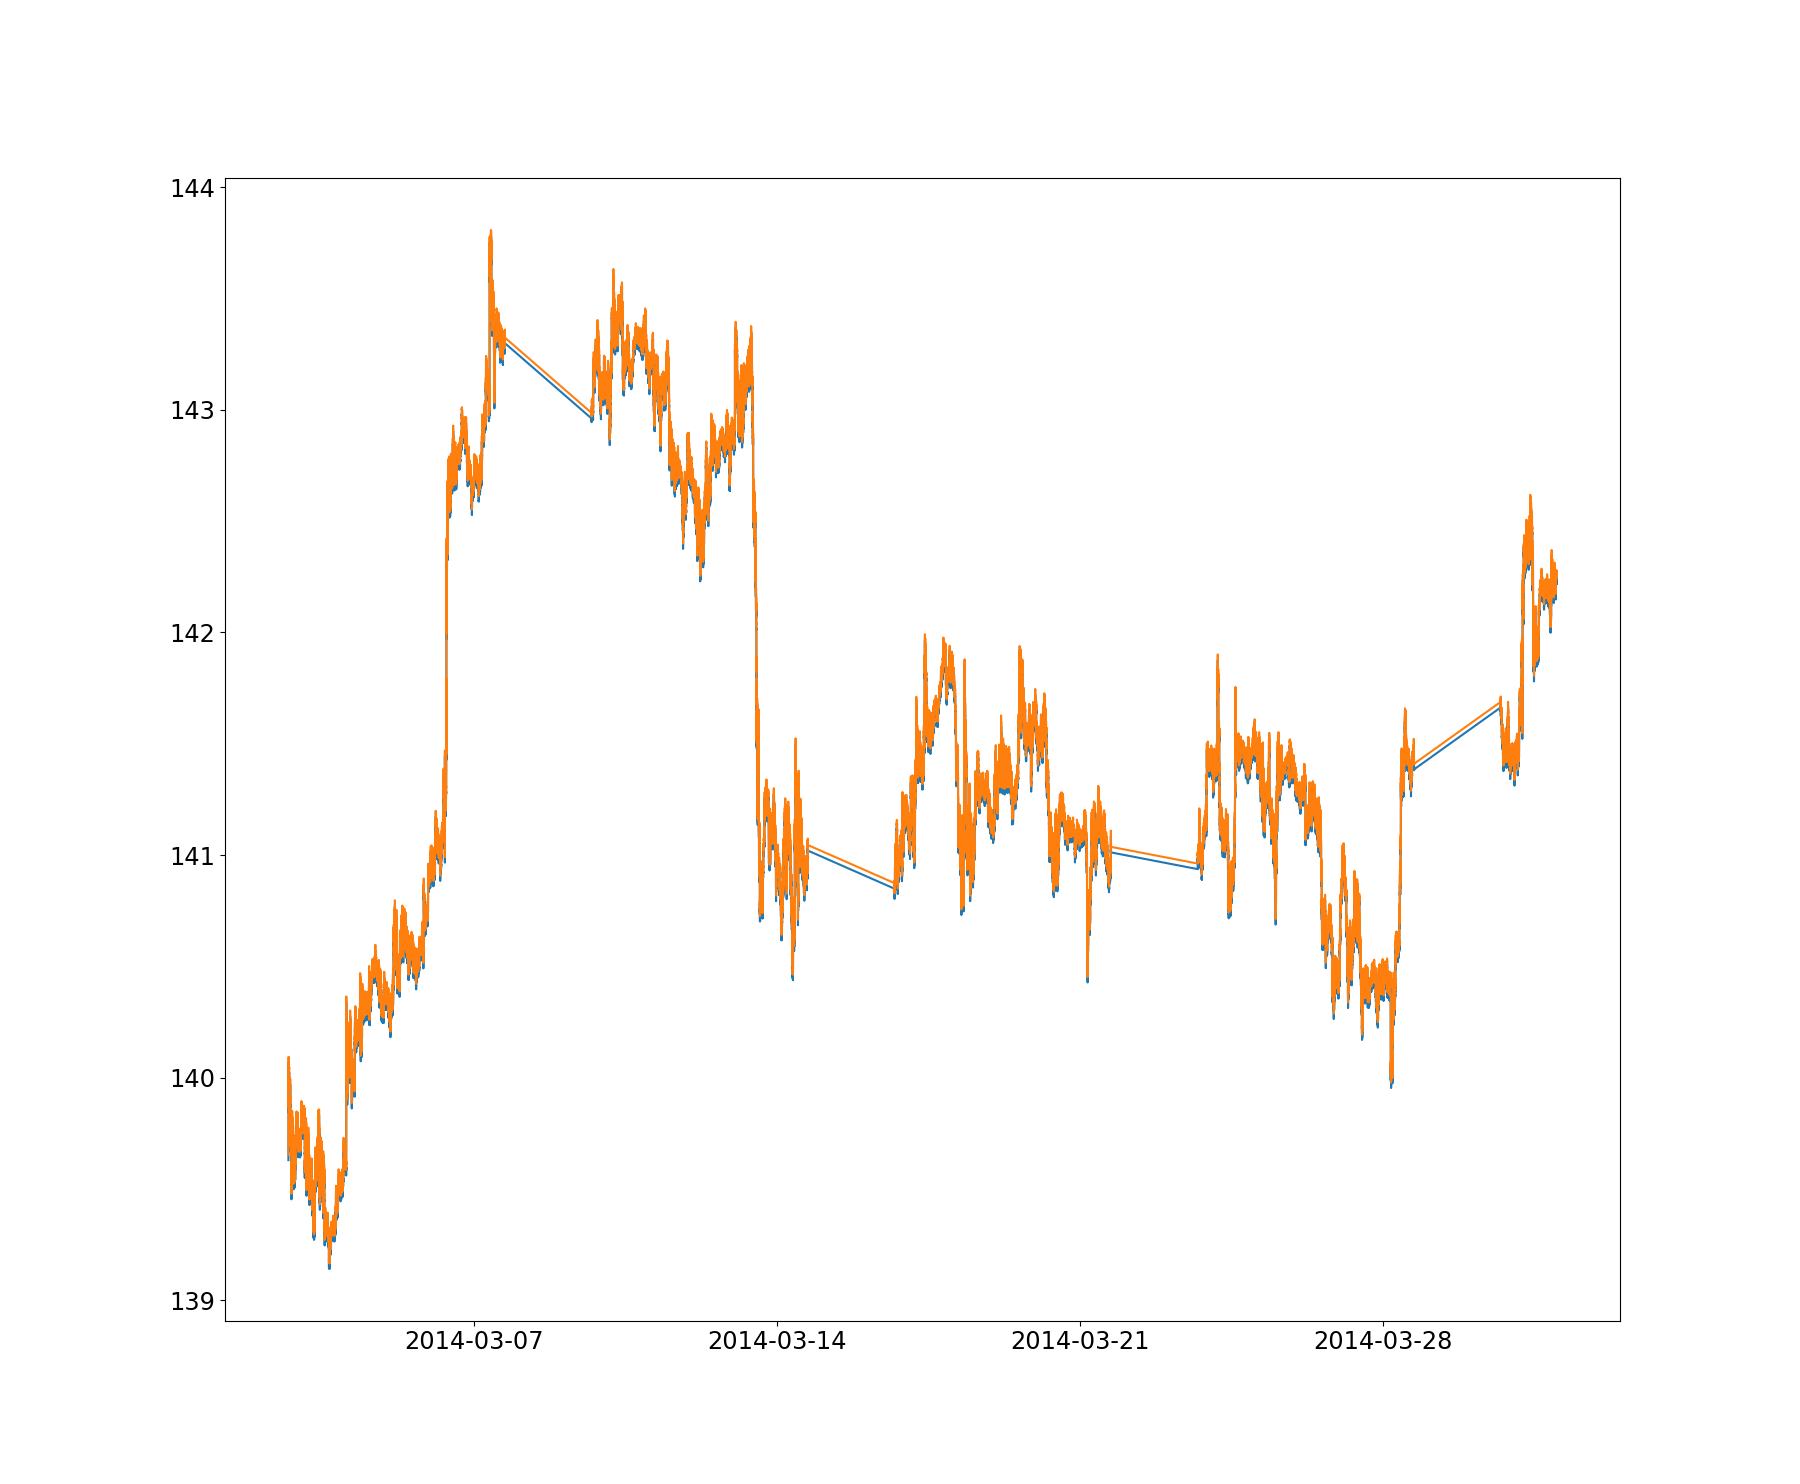
\includegraphics[width=\linewidth]{Figures/strat_1_bad_jpy_14_03}
		\captionof{figure}{EURJPY, March 2014:\\bad month for our strategy}
		\label{fig:7}
	\end{minipage}%
	\begin{minipage}{.5\textwidth}
		\centering
		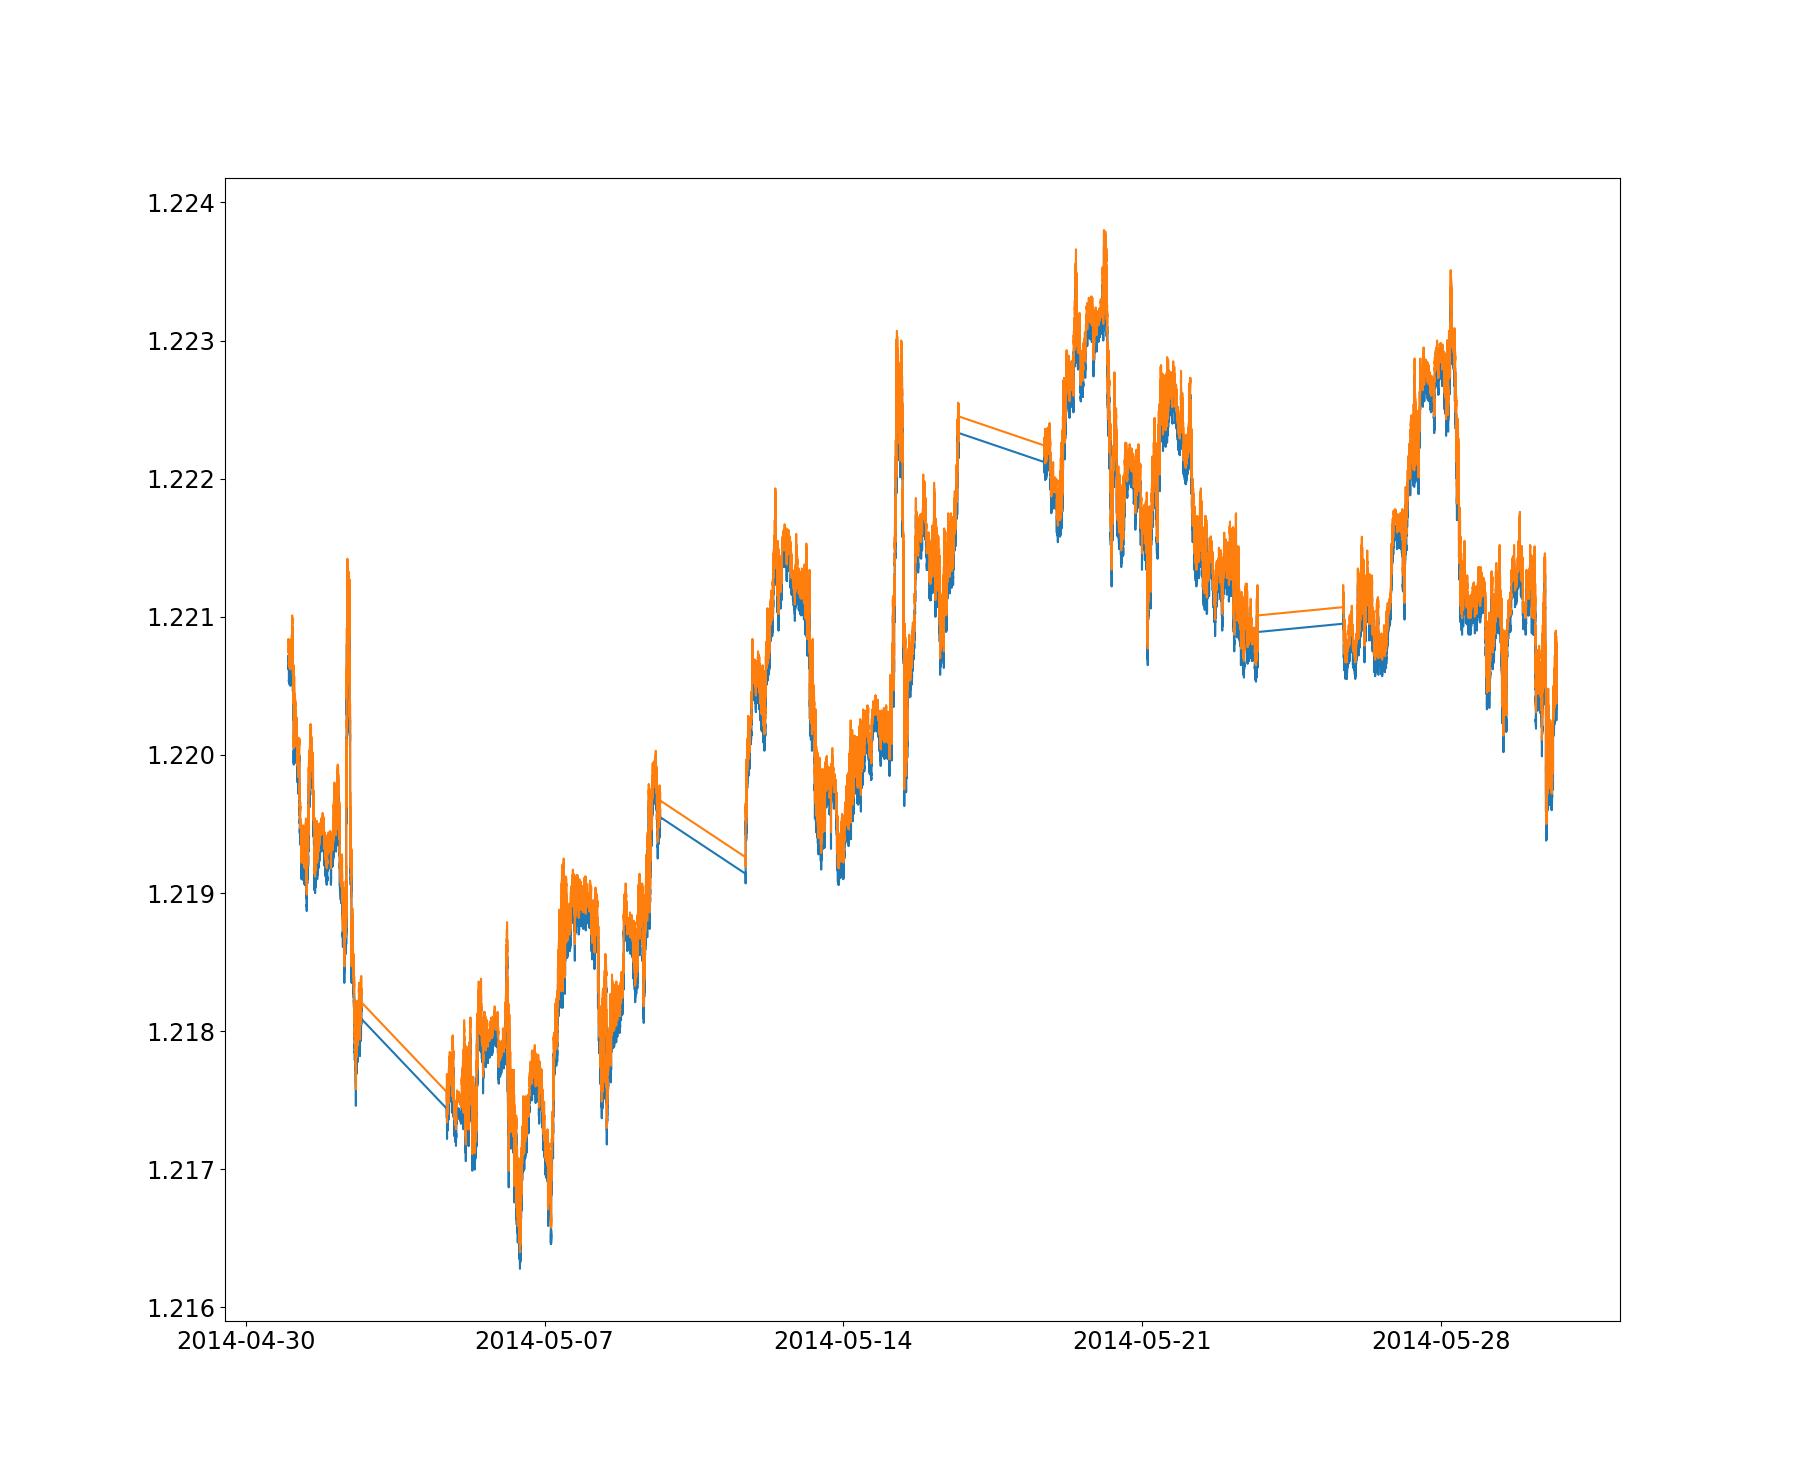
\includegraphics[width=\linewidth]{Figures/strat_1_good_chf_14_05}
		\captionof{figure}{EURCHF, May 2014:\\good month for our strategy}
		\label{fig:8}
	\end{minipage}
\end{figure}

\subsection{Implementation}

As it was said before, the idea behind this strategy is quite simple: when the price goes too high you short, when it goes too low you buy. The difficult part is how to understand if the price was too high or too low.\\
We did that by introducing a long-term mean and a short-term mean. When the difference between the two reached a threshold, we opened a position. We wanted the threshold not to be just a fixed amount, but to reflect the current volatility too. Computing the rolling standard deviation was not possible for our amount of data, so we used the spread as a proxy for it. Finally, the threshold was computed as a hard-coded multiplier times the spread.\\
To summarise, this is the core of our strategy:
\begin{verbatim}
      if (df['short_mean']-df['long_mean'] >  df['spread']*multiplier) ---> SHORT
      if (df['short_mean']-df['long_mean'] < -df['spread']*multiplier) --->  LONG
\end{verbatim}
We fixed the windows for the long-term mean and the short-term mean to 500 and 3, respectively. Once the strategy was triggered, we would hold the position for a fixed amount of data points (80) or until an opposite action was triggered.\\
The multiplier was decided once a year, based on what would have worked the best in December of the year before. We ranked the performance based on the cumulative return. The multiplier could vary between 3 and 20.\\
This strategy was implemented to be able to handle the huge amount of data that we downloaded. In order to do that, we decided to use \emph{Dask}. This limited our possible actions, but the whole process took only 1 hour.

\subsection{Results}

Due to its simplicity and to the clear challenges that we presented above. The performance of this strategy was overall quite terrible. The pair EURJPY in particular was the one where we would have lost money every single year. We suspect that this happened because it is quite typical to find big jumps without recall in this series and this is not compatible with our strategy.\\
Interestingly, the performance, reported in Figure \ref{fig:9}, in the other currency pairs increased in magnitude over the years. It is overall quite negatively skewed, with frequent small gains and some sporadic very big losses (e.g. we can see the effect of Brexit on EURGBP). Since we are calibrating the multiplier only on past data, this could be considered already as an out-of-sample performance, but we had already explored this data so we labelled it as in-sample.\\
We decided to test our strategy out-of-sample for all the currency pairs except EURJPY and we reported the cumulative results in Figure \ref{fig:10}. Here, the training was done monthly on the data of the previous month. We were not surprised to find that their performance was not exceptional in this case too.


\begin{figure}[h]
	\centering
	\begin{minipage}{.5\textwidth}
		\centering
		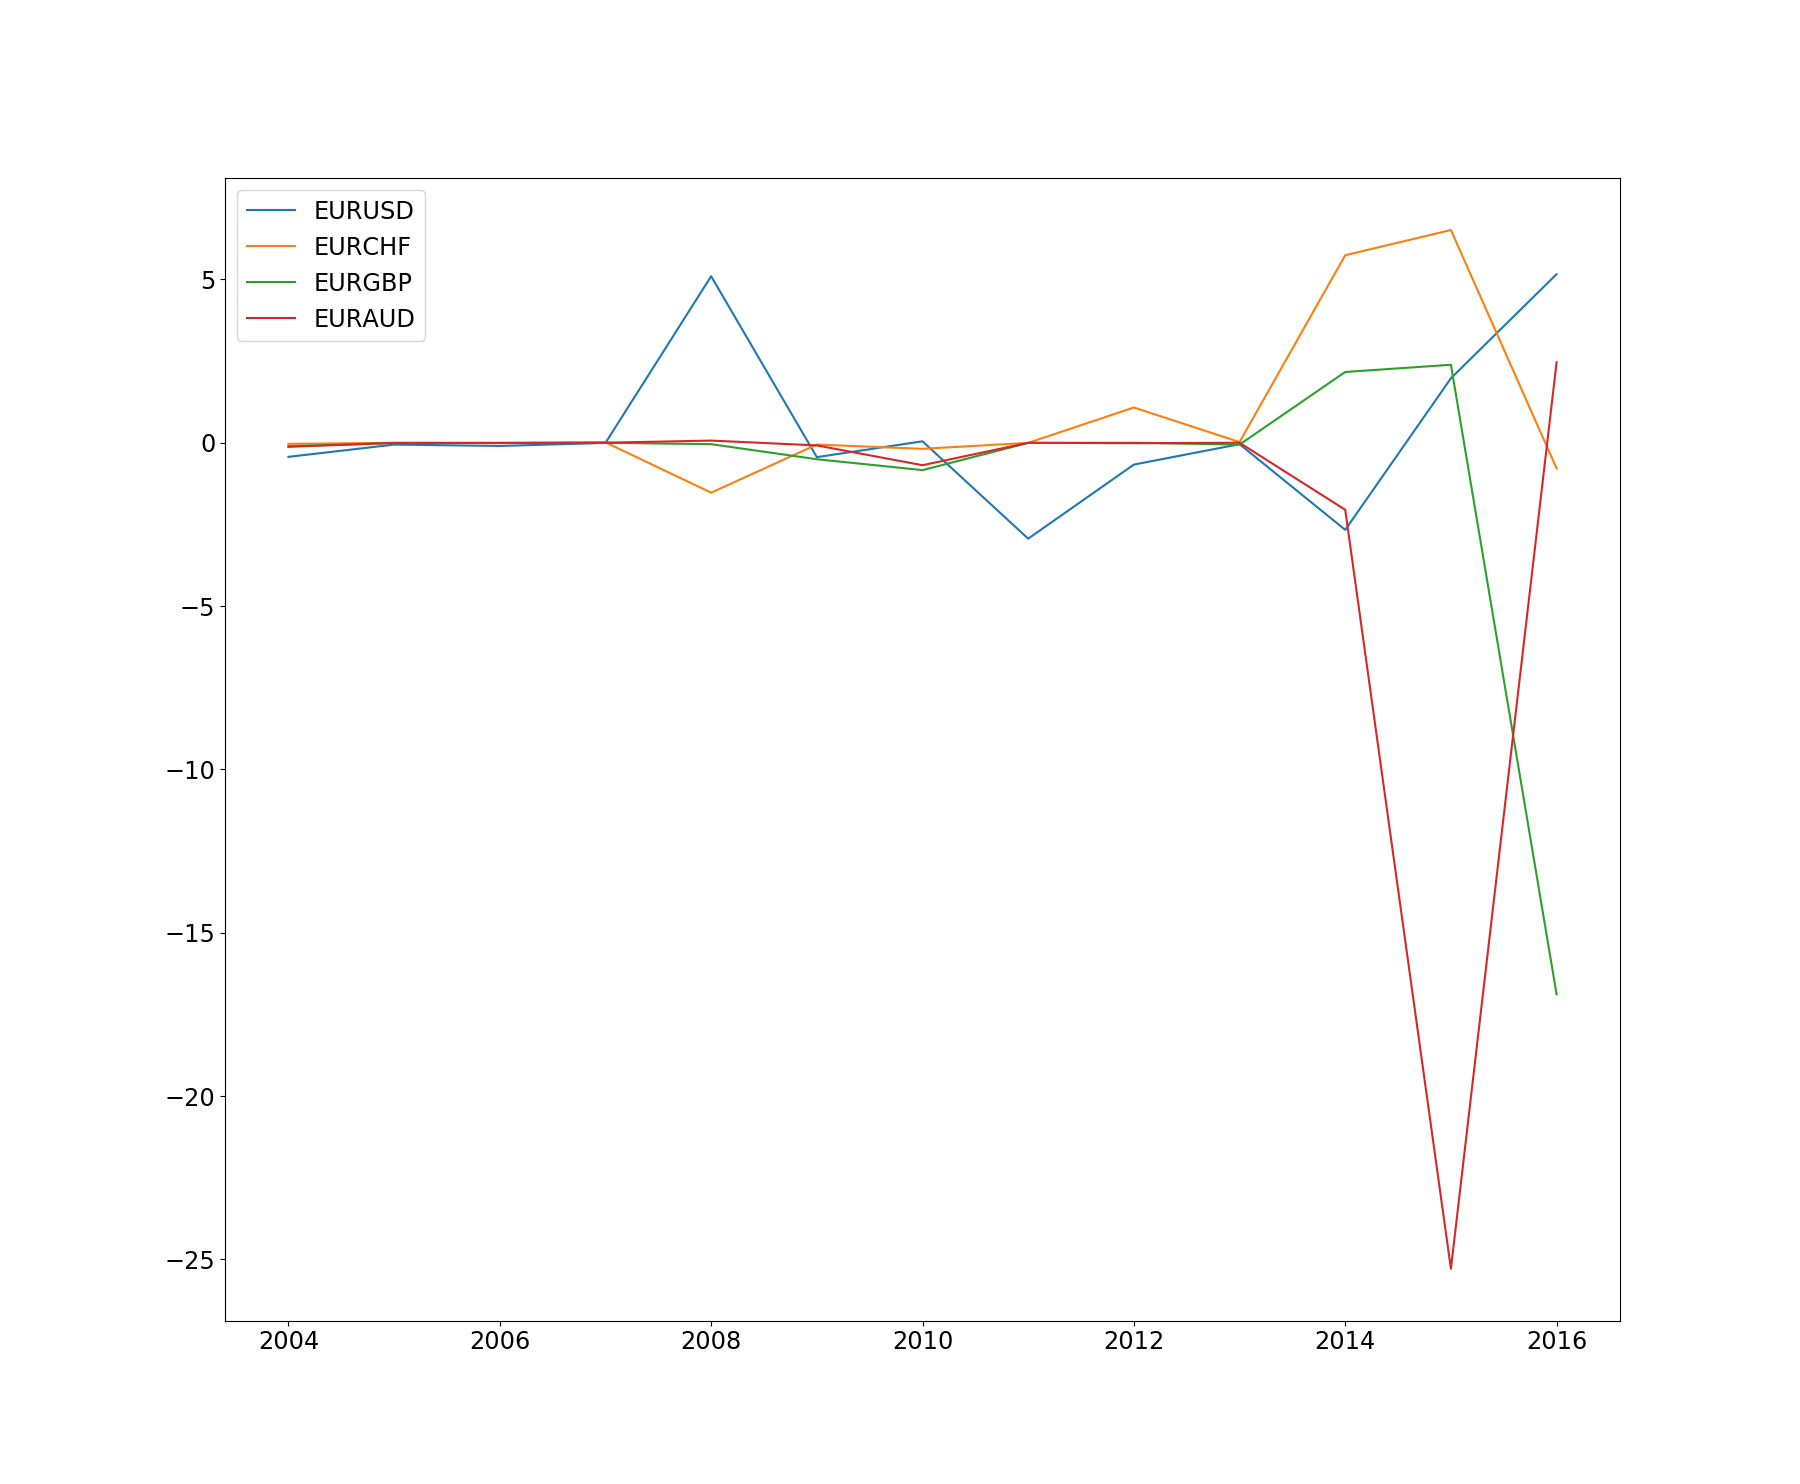
\includegraphics[width=\linewidth]{Figures/strat_1_performance_in}
		\captionof{figure}{Yearly in sample performance}
		\label{fig:9}
	\end{minipage}%
	\begin{minipage}{.5\textwidth}
		\centering
		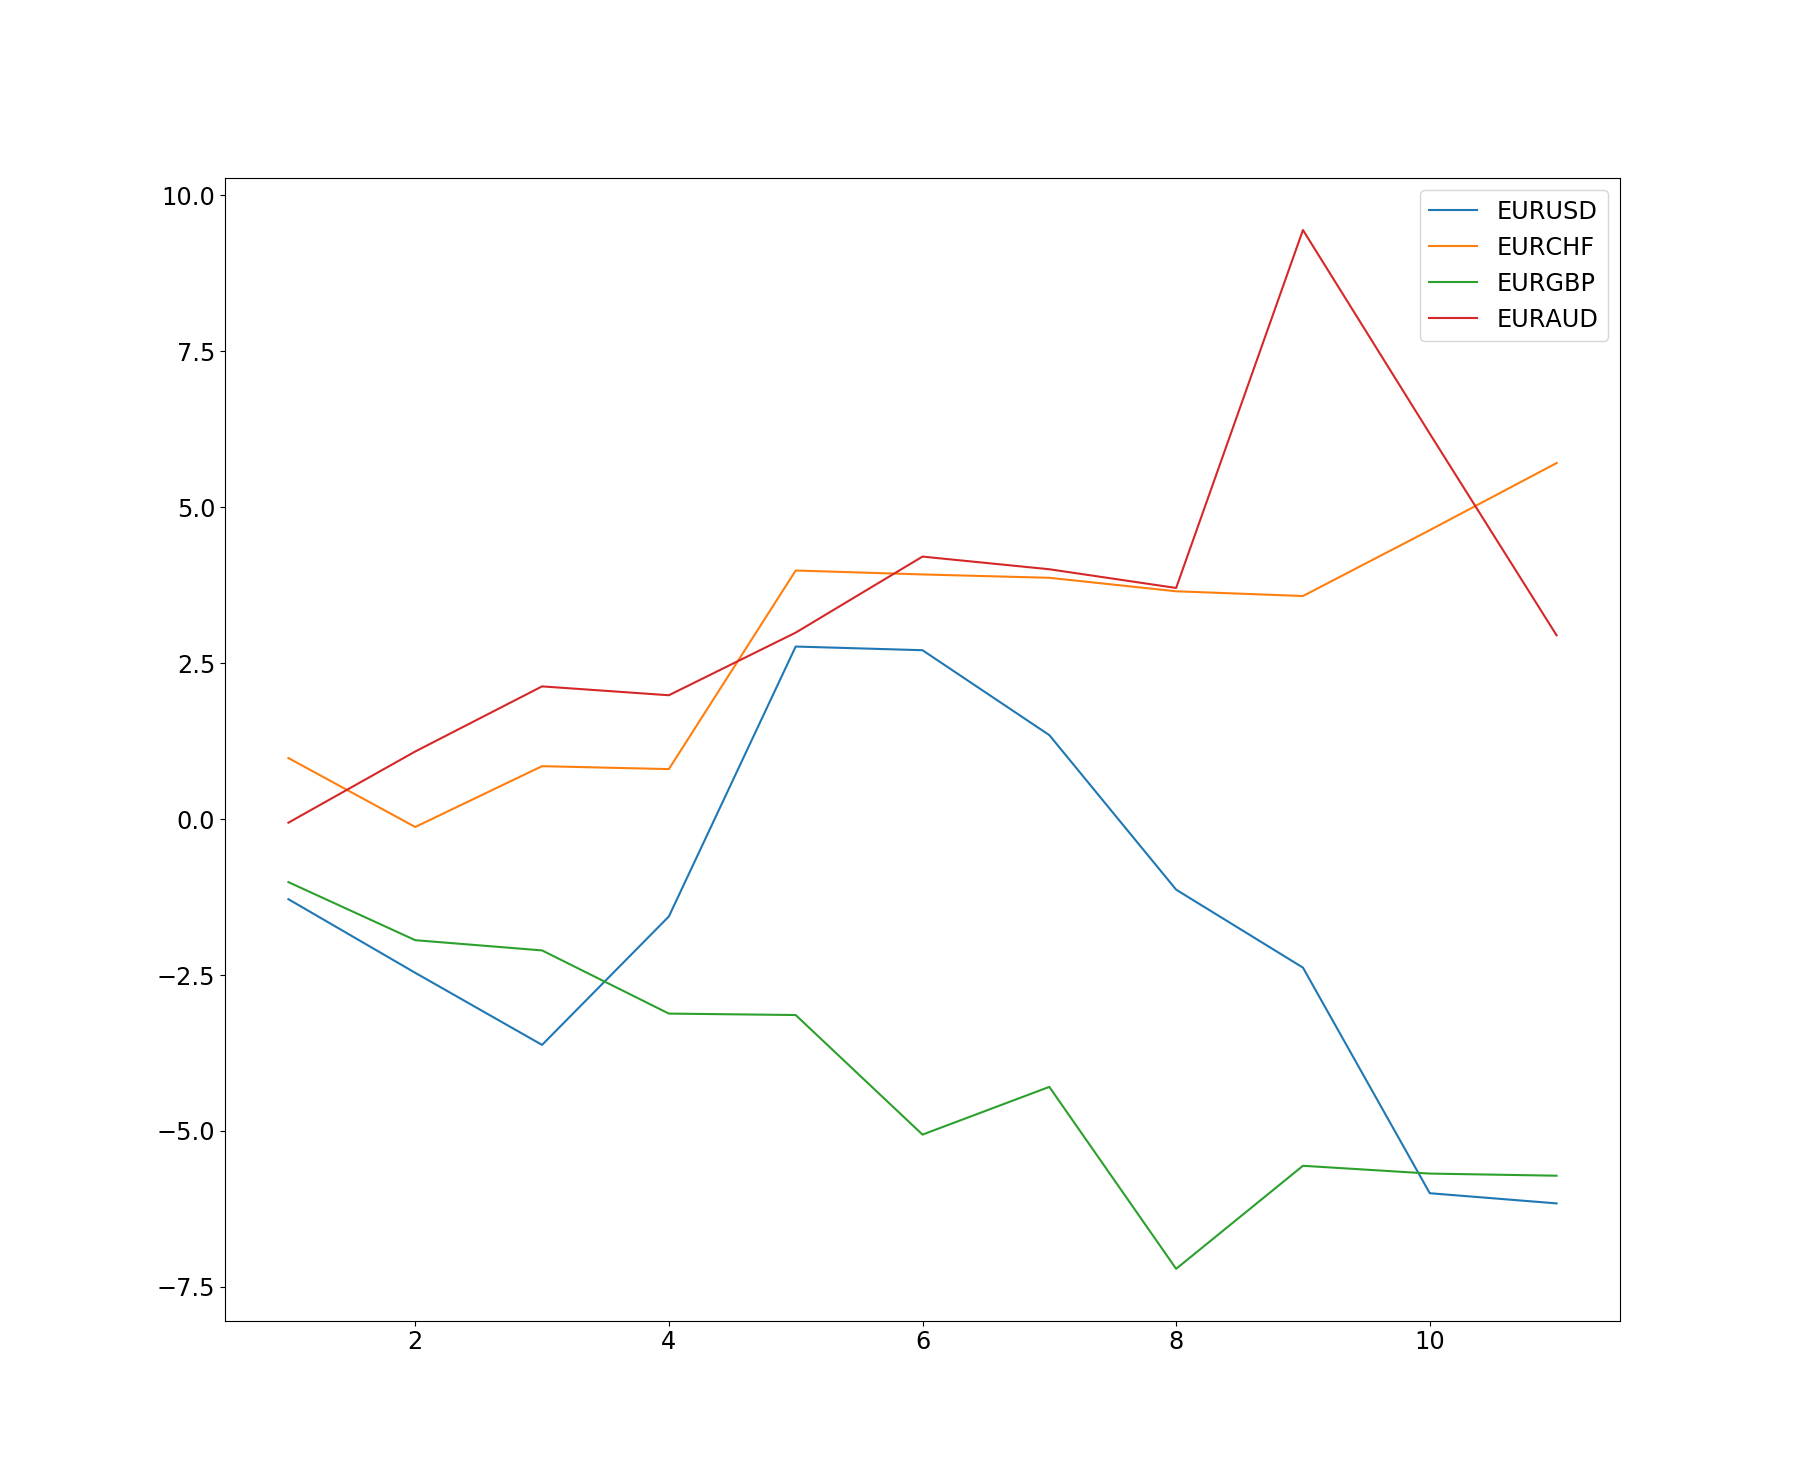
\includegraphics[width=\linewidth]{Figures/strat_1_performance_out}
		\captionof{figure}{Cumulative out of sample performance for 2017}
		\label{fig:10}
	\end{minipage}
\end{figure}

\subsection{Outlook}

There is definitely a lot that can be improved in this strategy. For instance, instead of holding the position for a fixed amount of data entries, we could have implemented two other thresholds: one where we exited if the strategy worked and a stop-loss threshold. However, the training time to find optimal amounts for those thresholds would have been too big.\\
Another big issue is that sometimes we are entering the position too soon and we are not profiting from the whole recall. Handling better the entering time would definitely improve the performance.\\
At the moment, we are only tuning the value of the multiplier. To choose the other parameters we compared the performance of the strategy in the first months of 2003. If they were allowed to evolve, there could be an improvement.\\
Finally, a mean reversion strategy essentially implies trading on noise and hoping that it will be reabsorbed. Currently, we are approximating the trend as the long-term mean and the noise as the difference between that and the short-term mean. This is clearly not the best approximation and, being at the heart of our model, it affects greatly its performance. We did it in this way because we were focusing our attention in developing a strategy that was computationally very efficient and able to crunch 14 years of tick-by-tick data in an hour. A smarter algorithm would have probably achieved a better performance at the expense of the computational time.



\section{30-minutes Strategy}

\subsection{Overview}

The idea behind the second strategy is deeply different from the underlying the high-frequency mean reversion strategy. Here we want to achieve positive returns with sophisticated and computationally intensive algorithms. To do so, we restrict our interest on a specific window of time from 2011 to 2017. The first thing we did, was to group tick-by-tick data into batches of 30 minutes, the result is a cleaner time series with insightful information about volatility, volumes (estimated as the number of trades occurring within the 30 minutes) and range. A 30-minute window seems to be a good trade off allowing to reduce the noise, but keeping a reasonable amount of data to train our predictive models. Each 30-minute entry of our dataset is identified by the first and last Bid-Ask quotes, a volume proxy a volatility measure and the min and max of the series (This part is done by the \textit{Group\_by\_Time.py} code).\\
The idea then is to use the data to train several models to predict the sign of the return and trade on this information. The algorithm is coded in a way that every month the model is re-trained on the previous 3 months of data so that out-of-sample progressively becomes in-sample as the window rolls in the future. We chose a 3-month window because it was the minimum amount of time that allowed to properly train the models incorporating only the most recent data, allowing to adapt quickly to changes in the market. One last crucial point is that the model and feature selection have been done on the first 6 months of data (January - June 2011) that have not been used in the backtesting results that will be presented later. In this way all the results are completely out-of-sample.

\subsection{Feature and model selection}

Accuracy was our favourite metric of performance assessment in our three-class classification problem $\{-1,0,1\}$.\\ Since we have to deal with relevant spreads we cannot afford to trade a lot and hope for a statistical edge to prevail. Therefore we chose to classify a return as belonging to the positive class ($\{1\}$) if it is bigger than the in-sample average positive return and negative ($\{-1\}$) if it is smaller than the in-sample negative mean. This way we have many returns belonging to class zero, but we also have a reasonable number of trades per month (5-10). Evaluating the performance of a model was not easy. Moreover, trying to do so while attempting at not only identifying the sign of the return but also the magnitude posed challenges in understanding which features could help us better predict. We tried to assess the impact of some crucial features by evaluating the improvement in accuracy and the importance metrics offered by a random forest tree. In the end, we used a big-data approach and put together a total of 80 different features. Some are just lags of returns, others are lags of volumes and volatilities. A couple of features that at the initial stages proved to be interesting are a Gaussian measure of returns:

$$
g_i = \frac{r_i - \mu_i}{\sigma_i}
$$

Where $\mu_i$ and $\sigma_i$ are the mean and standard deviation of the past 10 returns. Another interesting measure we wanted to include is the \textit{Relative Strength Index} that is an indicator that ranges from 0 to 100 and assesses the potential of the price to rebound. Typically a value of RSI below 30 and above 70 are respectively signs of respectively long and short potential. Another indicator that we used is just the difference between a short and a long exponential moving average of the price, this is supposed to give an idea of the ongoing trend. At last we considered some interaction measures that seemed to be really appreciated by Random Forest trees when training (of course, in the first 6 months not used in the backtesting).\\
Once the features are built, the dataset is standardized (all with in sample mean and variance), and the data is fed into a Gaussian Kernel PCA. In-sample we noticed that the Gaussian Kernel was the only one able to capture some relevant information. The only exception is represented by the EURUSD pair, where lower spreads made us choose a plain linear PCA because it gave more noisy results and allowed to trade more (in fact we have more trades on this currency). In the end we had 15 features.\\
For what concerns the model selection, we tried a different set of models, we opted in the end for the ones that in-sample prooved to be the more robust and precise. We decided to use a majority voting predictor, where the votes are given by a logistic regression, a gaussian kernel support vector classifier, a quadratic discriminant analysis and an AdaBoost classifier. The last two have the great adavantage that besides offering good in-sample accuracies, they prooved to be really resistent to changes in the features and amount of data given and in addition, they do not require hyperparameter tuning.\\ 

\subsection{Implementation}

The majority of the job here is done in an appropriate class (\textit{model\_class.py}).
This class is initialized with train and test set (they are different each month), then it fits the models on the given data (doing some hyperparameter tuning for the Logistic Regression and SVC), predicts the signs and trades. It also computes the raw and net PnL for each month. A couple of points here are worth mentioning:

\begin{itemize}
	\item Train and test are prepared separately, to avoid overfitting 
	\item All NaNs are dropped, so some hours cannot be traded
	\item The average returns are computed in-sample and then used out of sample to classify a return as 0,1 or -1
	\item Data is standardized just before the PCA is applied to get the maximum speed improvement.
	\item If a signal is given, we enter the position in the market at the first available bid or ask quote and we close the position at the end of the 30 minutes unless another signal of the same type is predicted (just a second before eventually closing a position), in such case we would keep the position opened for other 30 minutes.
\end{itemize}

The main backtesting code then calls the \textit{model\_class} each month backtesting on the previous three months.\\ Notice that the backtest starts on July 2011, because the first 6 months of 2011 were used to perform model and feature selection. Therefore, to be consistent we should not touch those 6 months in the Backtesting.\\

\subsection{Results}

We immediately excluded the EURJPY cross from the backtesting because from the in-sample test we noticed that spreads were extremely high, and moreover our model was not able to capture a significant amount of information from the data. For the other crosses, backtesting results (Raw Pnl and PnL net of spreads) can be found in Graphs 11 - 14.\\
It is clear how spreads really harm the ability of the model to make good trades. With a quick glance at the spreads, we noticed that these are significantly high (EURUSD offers a 4 pip spread in 2017 which is completely out of the market nowadays with brokers offering less than 1 pip spread or zero spreads on currency futures).\\


\begin{figure}
	\centering
	\begin{minipage}{.5\textwidth}
		\centering
		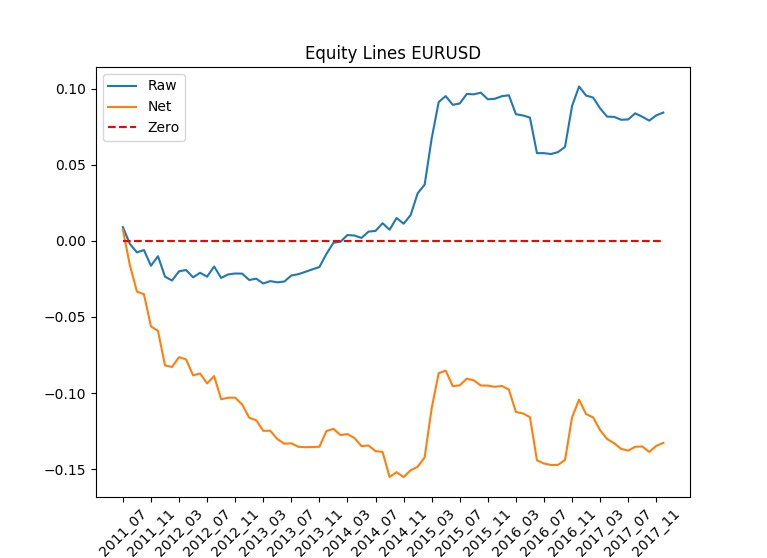
\includegraphics[width=\linewidth]{Figures/EURUSD.jpeg}
		\captionof{figure}{EURUSD Backtesting result}
		\label{fig:11}
	\end{minipage}%
	\begin{minipage}{.5\textwidth}
		\centering
		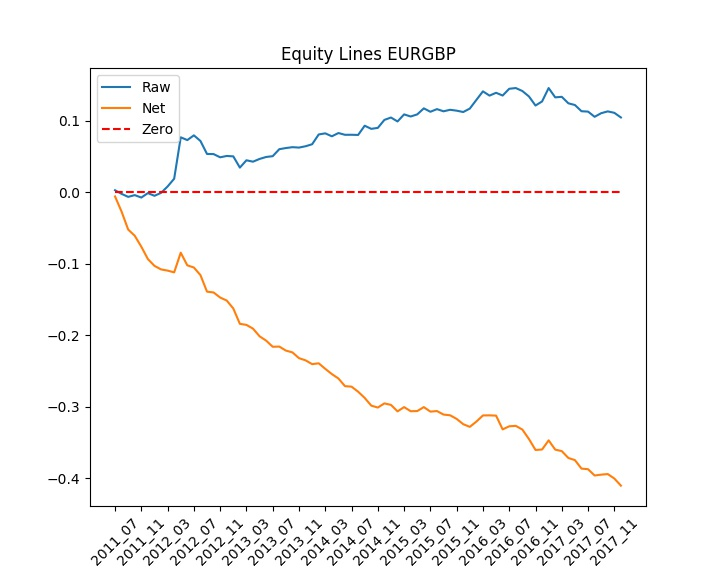
\includegraphics[width=\linewidth]{Figures/EURGBP.jpeg}
		\captionof{figure}{EURGBP Backtesting result}
		\label{fig:12}
	\end{minipage}
	\begin{minipage}{.5\textwidth}
		\centering
		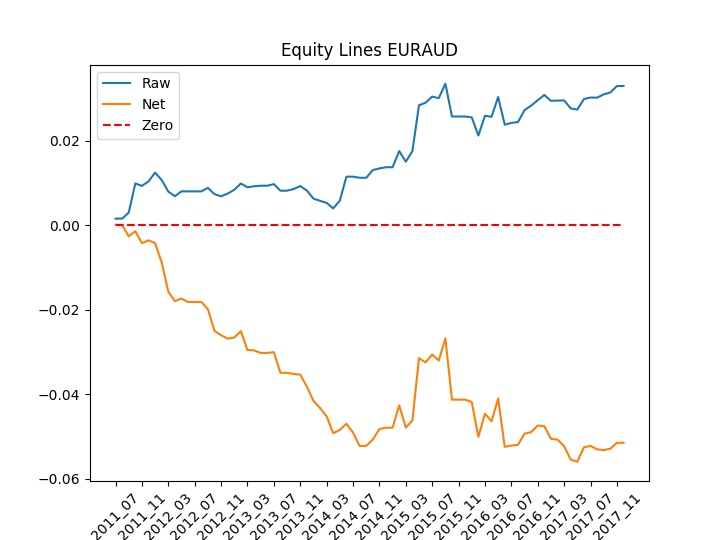
\includegraphics[width=\linewidth]{Figures/EURAUD.jpeg}
		\captionof{figure}{EURAUD Backtesting result}
		\label{fig:13}
	\end{minipage}%
	\begin{minipage}{.5\textwidth}
		\centering
		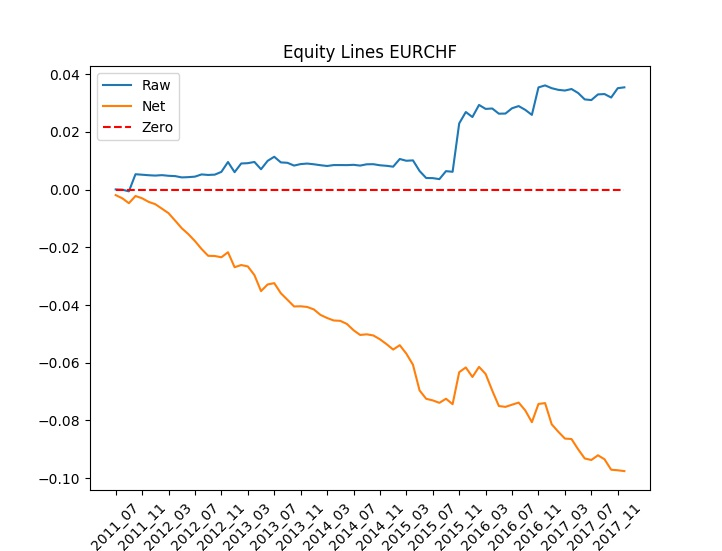
\includegraphics[width=\linewidth]{Figures/EURCHF.jpeg}
		\captionof{figure}{EURCHF Backtesting result}
		\label{fig:14}
	\end{minipage}
\end{figure}

As said before high spreads offset the job done by the models in predicting the signs of returns. We can see how the net performance of the strategies is related to the bid-ask spread, the higher the spread (and the number of trades) the worse the performance. For the EURGBP cross despite the spread is reasonable, we trade too much, paying a lot in transaction costs.\\

%\begin{figure}
%\centering
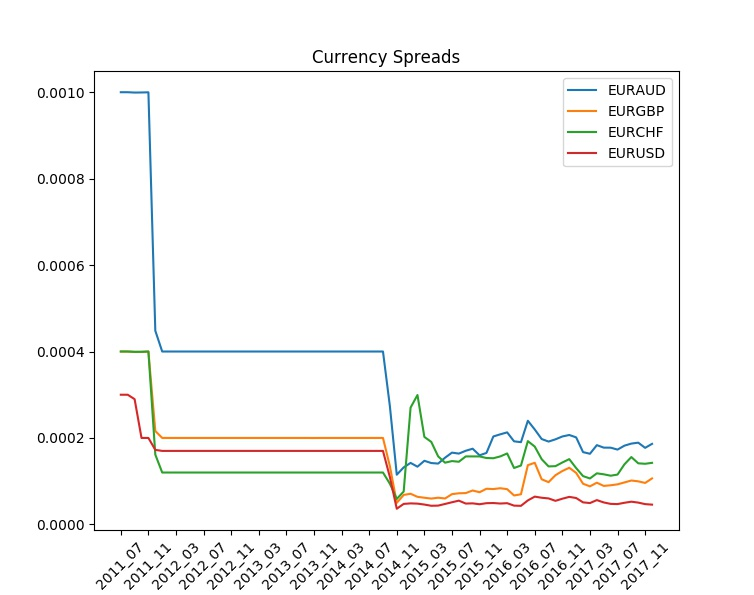
\includegraphics[width=\linewidth]{Figures/Spreads.jpeg}
\captionof{figure}{Spreads Evolution}
\label{fig:15}
%\end{figure}
\vspace{10pt}


	
Moreover, there is a time-effect, in the recent years spreads have definitely tightened making some strategies slightly profitable.\\
At last, we also tried to see how an allocation of the strategies together could perform (we apply this only to the net performance, because with such negative net performances it would make no sense to do so). We implemented both an equally weighted and a risk parity allocation (weights in the portfolio are inversely proportional to variance). The second allocation is created with a 6-month rolling window where we estimate variance of each cross to build the portfolio. (This part is done in the \textit{Portfolio\_perf.py} code), results are in Figure 16.

%\begin{figure}
%\centering
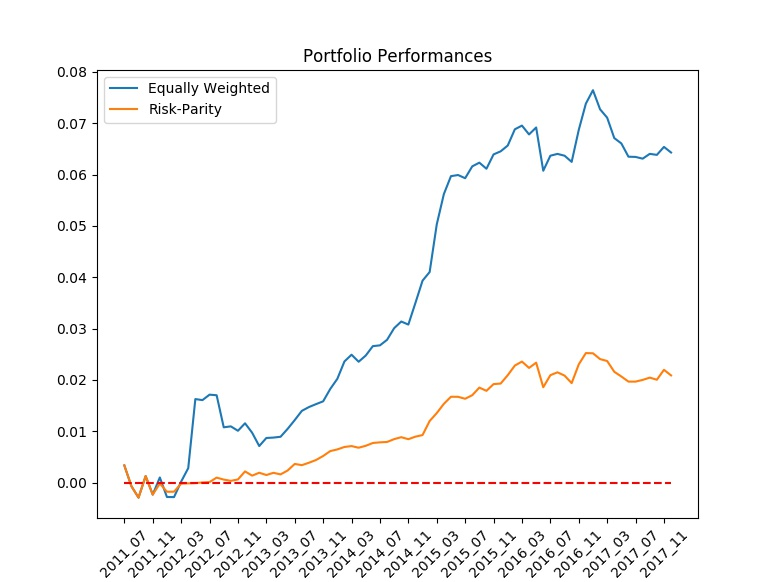
\includegraphics[width=\linewidth]{Figures/Portfolios.jpeg}
\captionof{figure}{Portfolios Backtesting result}
\label{fig:16}
%\end{figure}
\vspace{10pt}

	
As we can see the portfolio approach smooths a bit our equity lines, bringing the sharpe ratio up to 0.2674.\\


\subsection{Potential Improvements}

The first thing to improve the strategy would be to look for smaller spreads. This is crucial, because with less restrictive criteria to enter a trade (i.e. more trades per month) the raw PnLs significantly increased. We followed this approach in the EURUSD pair, but still we could be more aggressive on the currency.\\
Other improvements are in the area of position targets, we might have considered using take profits instead of keeping a position opened for strictly 30 minutes. This would have led on additional optimization and therefore we left it aside. Anyway we are confident that this could bring additional gains to our strategy.\\


\end{document}